% {{{ Preamble
\documentclass[pdftex,12pt,a4papaer,twoside,notitlepage]{report}
\usepackage[toc,page]{appendix}
\usepackage{geometry}
\usepackage[pdftex]{graphicx}
\usepackage{parskip}
\usepackage[numbers]{natbib}
\usepackage{url}
\usepackage{amsmath}
\usepackage{amsfonts}
\usepackage{setspace}
\usepackage{paralist}
\usepackage{enumitem}
\usepackage[]{units}
\usepackage{tabto}
\usepackage{float}
\usepackage{framed}
\usepackage{comment}
\usepackage{array}
\usepackage{titling}
\usepackage{hyperref}
\usepackage{cleveref}
\usepackage{todonotes}
\usepackage{textcomp}
\usepackage{listings}

% }}}

\setlength{\marginparwidth}{3cm}
\setcounter{secnumdepth}{6}
\setlist{nosep}

\crefname{section}{\S}{\S\S}
\Crefname{section}{\S}{\S\S}

\raggedbottom

\setstretch{2}


\title{DRACL}
\author{Steven Allen}
\date{August 31, 2016}

\newcommand{\note}[1]{\vspace{1em} \begin{spacing}{1}\textit{\textbf{Note:} #1}\end{spacing}\vspace{1em}}
\DeclareMathOperator{\e}{\mathbf{e}}
\DeclareMathOperator{\dual}{\mathbf{Dual}}
\newcommand{\seq}[2]{\left(#2 \, \middle| \, #1 \right)}
\newcommand{\iprod}[2]{\langle #1,\,#2\rangle}

\lstset{
  language=C,
  basicstyle=\ttfamily,
  breaklines=true,
  upquote=true,
  captionpos=b,
  frame=single,	
}

\DeclareMathOperator{\ein}{\mathtt{EncInput}}
\DeclareMathOperator{\combine}{\mathtt{LCombine}}
\DeclareMathOperator{\hash}{\mathtt{Hash}}
\DeclareMathOperator{\eins}{\mathtt{EncInputS}}
\DeclareMathOperator{\eouts}{\mathtt{EncResultS}}
\DeclareMathOperator{\pair}{\mathtt{Pair}}
\DeclareMathOperator{\hmac}{\mathtt{HMAC}}

\begin{document}

\newgeometry{left=1in,right=1in,top=1in,bottom=1in}

\begin{titlingpage}

  \begin{singlespacing}

    \setlength{\parskip}{1em}
    \begin{center}

      \textbf{DRACL (Decentralized Resource Access Control List)}

      by Steven D. Allen

      S.B, C.S. M.I.T. 2014

      \vspace{2em}

      Submitted to the

      Department of Electrical Engineering and Computer Science in
      Partial Fulfillment of the Requirements for the Degree of

      Master of Engineering in Electrical and Computer Science

      at the

      Massachusetts Institute of Technology

      August 2016

      \copyright~2016 Steven D. Allen. Some rights reserved.

      The author hereby grants to M.I.T. permission to reproduce and distribute
      publicly paper and electronic copies of this thesis document in whole and in
      part in any medium now known or hereafter created.

      \vspace{3em}
      \begin{tabular}{c l}
        Author: & \hrulefill \\
                & {\small Department of Electrical Engineering and Computer Science } \\
                & {\small August 31, 2016 } \\
        \\
        Certified by: & \hrulefill \\
                & {\small David Karger, Professor, Thesis Supervisor } \\
        \\
        Certified by: & \hrulefill \\
                & {\small Vinod Vaikuntanathan, Professor, Thesis Supervisor } \\
        \\
        Accepted By: & \hrulefill \\
                & {\small Dennis M. Freeman, Chairman, Masters of Engineering Thesis Committee } \\
      \end{tabular}
    \end{center}

  \end{singlespacing}

\end{titlingpage}

\cleardoublepage

\thispagestyle{empty}

\begin{singlespacing}

\begin{center}
    \vspace*{\fill}
    {%
        \onehalfspacing{} \bfseries \Large
        DRACL (Decentralized Resource Access Control List) \\
    }

    \vspace*{\fill}
    {\large
    \begin{minipage}{0.9\textwidth}
        \emph{Author:} \theauthor{} \hfill \emph{Advisor:} David Karger
        \\
        \begin{center}
              \thedate{}
        \end{center}
    \end{minipage}
    }

    \vspace*{\fill}

    \begin{minipage}{0.8\textwidth}
      \small
      \begin{center}
        In Partial Fulfillment of the Requirements for the Degree of Master of
        Engineering in Electrical Engineering and Computer Science.
      \end{center}

    \end{minipage}

    \vspace*{\fill}

\end{center}


\begin{abstract}
  DRACL is a \emph{privacy-preserving}, scalable, secure, and developer and user
  friendly federated access control system. It allows producers to manage,
  through a single authentication provider, which consumers can access what
  content across all content hosts that support the DRACL protocol. It preserves
  user privacy by not revealing the producers' social networks to content hosts
  and allowing content consumers to access content anonymously. Unlike existing
  solutions, DRACL is federated (cf. Facebook Connect, Google Sign-In), does not
  have a single point of failure (cf. Mozilla Persona, OpenID), and does not
  reveal its producers' social networks to content hosts (cf. Facebook
  Connect's~ \verb=user_friends= permission).
\end{abstract}

\end{singlespacing}

\restoregeometry

\cleardoublepage

\tableofcontents

\cleardoublepage

\setlength{\parskip}{1.5em}
                                              
\chapter{Introduction} 

Today, the web is basically a big social network. Producers --- users who post
content --- post content on various content hosts (e.g., Facebook) while
consumers --- users who access content --- interact with this content on these
various content hosts. This really is an amazing system that allows people to
interact socially across barriers that were previously insurmountable (e.g.
distance, culture, and social status).

Unfortunately, these content hosts don't interoperate well and this lack of
interoperability introduces barriers to social interaction through both poor
usability and privacy issues. Poor usability directly bars communication by
making it harder. Privacy issues bar communication by discouraging users who
value their privacy from socializing on the web and encouraging those who do
socialize to self-censor.

While all users could simply sign up for the same monolithic service, this is
inherently bad for privacy. The monolithic service can do pretty much whatever
it wants and get away with it because there is no competition. Therefore, users
will either self-censor or choose to simply not socialize online. Unfortunately,
this is what we have today with Facebook.

On the other hand, if users choose to use diverse content hosts, the lack of
interoperability becomes a social barrier. For one, consumers need to have
accounts on every content host used by their friends. This is a usability
problem because it forces users to manage multiple accounts and a privacy
problem because content hosts often require that account holders sign up with
their ``real'' names. Additionally, producers need to recreate their social
networks on every content host. This is also usability problem because it forces
producers to manage their ``friends list'' in multiple locations and is also a
privacy problem because it forces producers to share their ``friends list'' with
multiple services.

In this thesis, we propose a privacy-preserving, scalable, secure, user and
developer friendly web-wide federated access control scheme that solves a
significant portion of this problem. Our system allows producers to share
content with consumers without having to manually recreate their ``friends
list'' on every service they use regardless of what content hosts their friends
use. Furthermore, it allows consumers to anonymously access any content shared
with them on any content host.

\section{The Big Picture}

In this section, we look at the bigger picture to understand where our access
control system fits into our dream of how the web should look.

\subsection{The Dream}

The web should look like one big interconnected social network. People should be
able to share with anyone on any host regardless of whether or not said person
has an account with any specific host. Additionally, people should be able to
access material shared with them without having to jump through hoops, sign up,
or hand out personal information to the website hosting the content. It should
be a web without walls.

It should be user friendly. People shouldn't have to manage multiple accounts or
manually re-create their social network on every service they use.

It should be free and fluid. People should be able to choose what services they
use, where they host their content, and how they communicate. They should be
able to move from service to service and even communicate across multiple
services without fragmenting their social networks.

It shouldn't require users to sacrifice their privacy in order to participate.
People should be able to access content shared with them without being forced to
give up personal information. People should be able to share content without
revealing their social network to the party that happens to host the content.

It should be secure and robust. A single service going down shouldn't shutdown
social communication online. A compromise of a single service shouldn't lead to
a cascading compromises of other services.

\subsection{Reality}

The web does not look like one big interconnected social network. Instead, it's
filled with walled off ``social networks'' that don't interoperate by design.

It's not user friendly. Users must manage multiple accounts. Some smaller
services give users the option to authenticate with one of a few ``blessed''
third-party accounts but these aren't standardized and don't give the user the
freedom to choose who they trust (they have to choose from a small set).

It's not free and fluid. Someone on Google+ can't share content with someone on
Facebook. This fragments social networks and forces people to stick with
services they may not like simply because that's where their friends are.

It impossible to socialize with friends and family online without sacrificing
privacy. For example, Facebook requires anyone wanting to simply access content
to have an account and requires that all account holders sign up with their real
name. On a web without walls, people should be able to access content shared
with them on, e.g., Facebook without ever signing up or telling Facebook
anything about themselves.

It's not secure and robust. Shutting down Twitter and Facebook effectively shuts
off most social interaction on the web. A compromise of Facebook would
compromise most semi-private social interactions on the web and would compromise
all websites that use Facebook's authentication service, Facebook Connect.

\subsection{Dissecting The Problem}

We've broken this dream into four building blocks: content hosting, identity
management, access control, and content notification. Here, we only tackle
access control but it helps to understand the bigger picture.

\subsubsection{Content Hosting}

Content hosting addresses the problem of storing content and social media
interactions. To interact online, people need a place to store their
interactions. That's the content host's job.

The problem of hosting content has been solved; this is the web as-is. People
can already choose from a plethora of content hosts such as Facebook, Flickr,
Google+, Twitter, Google Docs, etc. The existing solutions aren't always
perfect: it's still very hard for people to move their content from one content
host to another. However, this is slowly being fixed by data export tools (e.g.,
Facebook's ``Download Your Information'' service).

\subsubsection{Identity Management}

Identity management addresses the problem of naming someone on the internet.
Identity management is a prerequisite for any social network that isn't entirely
public (e.g. 4chan) because a producer needs to be able to name, or describe, a
consumer to state whether or not that consumer should be able to access
something. In our case, we need an identity management solution that allows
naming people across services.

Many systems attempt to address the identity management problem. These include
Facebook Connect, Keybase, NameCoin, and GnuPG (OpenPGP). Unfortunately, none of
these are perfect: Facebook is completely centralized, Keybase is somewhat
centralized, NameCoin is untested and complicated, GnuPG's user experience is
needlessly complicated (it usually requires manually comparing long key
fingerprints and mucking around with arcane command invocations), and none of
the decentralized systems have wide adoption. However, this \emph{is} a well
explored problem lacking only a simple, widely adopted decentralized solution;
probably because there isn't much use for one at the moment outside of sending
encrypted email.

\subsubsection{Access Control}

Access control addresses the problem of limiting who --- identified by the
identity system --- can access what. To make the web look like one big social
network, we need an access control system that can limit access to content
independent of where it is stored.

There really aren't any systems that generically address the problem of access
control problem. For example, there's no way to tell Flicker ``allow my
classmates to access this photo album'' unless Flicker has an explicit list of
your classmates and they all have accounts on Flicker. There are federated
social media platforms like Diaspora and that allow this kind of cross-platform
interoperability; however, these kinds of systems usually attempt to solve all
four problems at once. This means they \emph{can't} be used with any of the
existing content hosts without requiring extensive modification to these content
hosts. This would require re-building the web from scratch and throwing away
what we already have.

\subsubsection{Content Notification}

Content notification (or publish-subscribe) addresses the problem of consumers
learning about content they can access. Conversely, it allows publishers to
notify consumers about content. We need this because, while an access control
system can permit or deny a consumer's access to content, it doesn't actually
tell the consumer where to find content they can access. In Facebook terms, this
is the \emph{status}/\emph{feed}. To achieve our goal, we need a content pub-sub
system that allows producers to advertise content to consumer independent of
where it is stored or where those consumers have accounts.

There are some pretty decent decentralized web-wide pub-sub systems although
many of these systems aren't widely adopted. The current most widely adopted
decentralized solution is email --- although email the ``sub'' part of pub-sub
doesn't really apply to anything but mailing lists. However, people tend to get
more email than they can handle anyways. Better solutions are systems like RSS
or even distributed Twitter-like systems such as pump.io\cite{pump.io}.

\subsection{Our Contribution}

In this thesis, we address the access control problem. We design a
privacy-preserving, scalable, secure, user and developer friendly access control
system for the web that allows producers to manage groups of consumers and
declare which groups can access what content what content across all content
hosts that use DRACL through a single authentication provider chosen by the
producer. Additionally, our system preserves privacy by hiding the producer's
social network from both content hosts and consumers and it by allowing
consumers to access content anonymously.

We build our access control system on top of the web as it is. Therefore, we can
use the existing rich ecosystem of content hosts without having to re-build the
web from scratch.

We assume that the web will eventually standardize on a single identity
management system. We've designed our access control system to work on top of
any identity system as long as this identity system is able to map identities to
cryptographic keys. Keybase has demonstrated that pretty much all identity
systems can do this in some form or another through the use of special
cryptographic proofs.

We also assume that the web will eventually standardize around some reasonably
small set of content notification protocols. There are plenty to pick from, it's
just a matter of adoption.

While we're still a ways off from a web without walls, we provide a large
missing component and were able to do so without redesigning the web from
scratch.

\section{Terminology}

Before actually diving into the problem of access control and our solution, we
need a consistent, well defined language for discussing it. Below, we define
some critical terminology used in this document.

\begin{compactdesc}
    \item[Identity] An assumed identity. That is, identities may not correspond
      one-to-one to real people. They may be pseudonymous, or may correspond to
      groups of people.
    \item[Producer] A user that publishes content and wishes to control
      access to said content.
    \item[Consumer] A user that accesses content.
    \item[Authorized Consumer] A consumer that is authorized to access a
      particular resource.
    \item[Group] A group of users as defined by a producer. In DRACL, groups
      are the unit of access control (i.e., producers grant access to groups,
      not directly to individual consumers).
    \item[Authentication Provider (AP)] A helper service for facilitating access
      control. Every DRACL producer will have an AP (just like every email user
      has an email provider). Basically, the AP can perform limited actions on
      behalf of producers while they're offline and can help ensure that a
      compromise of a producer's account is recoverable. We assume that the AP
      isn't actively malicious but can be compromised and may be nosy.
    \item[Content Host] A website/service using this system to authenticate
      content it hosts. For example, Flicker, Facebook, Imgur, etc.
    \item[Friend] Same as a Facebook friend. That is, the relationship may or
      may not be friendly.
    \item[Honest But Curious Party] An honest but curious party follows
      protocols as specified but attempts to learn information they shouldn't
      know by looking at the protocol's trace. That is, they aren't actively
      malicious, just nosy. This is the standard cryptographic definition of
      honest but curious.
    \item[Malicious Party] A malicious party, on the other hand, will deviate
      from the protocol when convenient.
\end{compactdesc}

\section{Requirements}

We would like a privacy-preserving, user and developer friendly, secure, and
scalable access control system for the web that promotes user freedom. In this
section, we discuss what these requirements mean in the context of access
control systems and why we care about them. We make no assumptions about whether
or not such a system already exists; we simply state what we want out of such a
system.

Two explicit non-requirements are hiding the content from content hosts and
hiding metadata --- who's communicating with whom --- from global adversaries
such as governments. These goals are simply out of scope of an access control
system. The first can be provided by simply encrypting the content and the
second and can be provided by a dedicated metadata-hiding anonymous
communication system like Vuvuzela~\cite{vuvuzela}. If you're looking for a
system that provides this functionality you're lost, look elsewhere.

We also expect that (authorized) consumers and producers will be honest but
curious, not actively malicious. At some level, discouraging ``bad'' behavior
becomes a social problem, not a technical problem.

\subsection{Privacy Preserving}

By privacy preserving we mean that a good access control system should avoid
revealing metadata. That is, it should reveal neither the identities or actions
of consumers nor the composition of its producers' social networks to any party
when possible.

First, such a system should not reveal the identities of consumers to content
hosts because people should not be excluded from social interactions for valuing
their privacy. In the web as it exists today, it's impossible to participate in
social networks without handing out personal information to third parties. This
forces people to either hand out this information or isolate themselves
completely. While, to prevent abuse, social networks often need
producers/producers to identify themselves, we believe that consumers should be
able to access content without identifying themselves. This would allow people
to anonymously access content on any content host while only publishing content
on content hosts they trust. While many consumers may choose to identify
themselves (e.g. by logging in), this should be by choice.

Additionally, such a system should also not reveal the identities of consumers
to content hosts because it would discourage the sharing and consuming of
content due to fear of judgment by association. Producers may choose not to
share a piece of content with a consumer because they don't want to be
associated with the consumer. Consumers may choose not to access a piece of
content because they don't wish to be associated with the producer. In general,
a good access control system should not influence what people share.

Second, such a system should not reveal the consumer activity to anyone,
especially producers. If a consumer views a piece of content, the content's
producer should not be notified in any way without the consumer's explicit
consent. Otherwise, the consumer loses the freedom to choose to either defer or
avoid participation in a social interaction. For example, if the fact that a
consumer has read an invitation were revealed to a producer, the consumer would
be pressured to out-right reject or accept the invitation instead of simply
pretending not to have seen it. This would force the consumer to either lie (``I
have plans''), do something socially unacceptable (reject it), or attend some
event they don't want to attend (potentially dangerous). Basically, how to
respond to a piece of content should be up to the consumer. However, we don't
believe that it's the access control system's job to prevent actively malicious
producers from subverting the protocol to learn this information. Such behavior
should be discouraged through social means and such producers are likely to have
a hard time making friends.

Finally, such a system should not reveal the structure of a producer's social
network, \emph{especially} to members of their social network, because would
again influence if and to whom a producer chooses to share content. People
should feel free to exclude others from their social network; the ability to
communicate privately (exclude unwanted parties) is necessary to prevent
self-censorship. For example, if an access control system revealed that two
consumers are members of some shared group while a third consumer is not, a
producer might feel pressured include all three in the same group to avoid
offending the third. This would, in turn, cause the producer to either share
content more widely than they might otherwise choose or refrain from sharing at
all (a chilling effect).

Privacy is an essential freedom for enabling the free expression of social
behaviors. Any information disclosure in a system limits the usefulness of that
system to social behaviors that can tolerate the disclosure of that information.
A web-wide access control system that doesn't protect user privacy would
therefore inhibit the types of social behavior applicable to the web. This is
not to say that all social behavior should be tolerated. However, it's not the
job of an access control system to limit social behavior.

\subsection{User Friendly}
\label{sec:goal-user}

By user friendly, we mean that sharing and accessing content across content
hosts should be as easy as sharing content on a centralized social network like
Facebook. Users shouldn't have to manage multiple sets of credentials or
manually recreate their social network on every content host they use.

Currently, content hosts (usually) force their users to manage one set of
credentials per service. In addition to being beyond annoying, this practice
encourages users to choose simple passwords or reuse them. A good global access
control system can eliminate this problem by allowing users to manage a single
access control account and re-use the same account from service to service.

Additionally, an access control system shouldn't assume that producers will run
their own servers or pay for anything. The amount of invasive advertising, poor
software, and privacy violations people tend to put up with on the internet for
``free'' services is a testament to how far people will go to avoid paying.

Finally, a user friendly access control system needs to support groups. Groups
allow producers to manage access to content at a level more coarse grained than
individual consumers but finer grained than ``all friends''. Without support for
groups, producers wishing to share with more than a few consumers are likely to
just share the content with all of their friends because manually selecting more
than a few users is extremely tedious.

Group support goes deeper than the UI. Adding/removing a consumer to/from a
group should retroactively grant/revoke that consumer's access to the group's
content. Otherwise, producers would have to manually grant/revoke access on a
content-by-content basis which would be extremely tedious. Worse, it's error
prone so a producer might forget to revoke a malicious consumer's access to some
piece of content.

Again, this comes back to reducing not limiting social interaction on the web.
Usability problems in an access control system turn into communication barriers
because users will choose not socialize in some way something because it's hard.
Therefore, a good access control system should try to stay out of the user's way
as much as possible and make socializing online as easy as possible.

\subsection{User Freedom}
\label{sec:goal-freedom}

By user freedom we mean that, a good access control system should enable users
to choose which online services they use and should allow them to freely to move
between them. This is closely related to both privacy and user friendliness as
it's a prerequisite for both but it bears discussing as a stand-alone category.

Currently, it's prohibitively difficult to move between content hosts because
because social networks are usually tied to a single content host. A global
access control system can alleviate this problem by allowing producers to grant
access to their friends on any content host regardless of what content hosts
their friends use.

A consequence of making it easier to move between content hosts is more
practical competition as it lowers the barrier for bootstrapping new services.
This is a direct consequence of allowing producers to share content with
consumers without forcing these consumers to create accounts. Competition is not
only good for users, it's absolutely necessary to keep companies from taking
advantage their users over in pursuit of higher profit margins. See
AT\&T\cite{att} policy and Comcast's\cite{comcast} recent attempt to charge an
additional fee for not snooping on their customers browser history.

Finally, a good access control scheme must be decentralized. We have an entire
section on this later (see \cref{sec:identity-auth}) but the short version is
that decentralized systems give users the ability to choose who they trust.
Forcing users to use the same authentication system would defeat the purpose of
allowing users to choose and move between content hosts. The centralized
authentication system would become the new Facebook.

\subsection{Secure}

By secure, we mean that only authorized consumers should be able to access
content, producers should be able to efficiently/reliably revoke access from
consumers, and compromises should be recoverable.

First, only authorized consumers, the content's producer, and the content host
should be able to access content, no ``trusted'' third parties. Currently, if
someone were to hack Gmail, they'd be able to access pretty much everything on
the public internet (through, e.g., password reset emails). This was a mistake.
Therefore, a good access control system should avoid this problem by design.

Second, for efficient and reliable revocation, a producer should not have to
contact every content host in order to remove a consumer from a group. First,
this would trigger a lot of up-front network traffic, even for old content that
may never be accessed again. Second, it would violate the fail-safe principle of
systems design: if a producer were unable to contact some of their content hosts
for some reason, there would be no way to revoke access.

Finally, no compromise of any single party should be unrecoverable and no
compromise of any single party should bring down the entire system. Websites are
hacked all the time and user account compromise is common so any system that
can't recover from compromise is dead in the water.

Users must feel safe socializing online. They must be able to rely on the fact
that even if something goes slightly wrong --- which it will --- their online
interactions will still, for the most part, be private and secure.

\subsection{Developer Friendly}
\label{sec:goal-developer}

By developer friendly, we mean that a good universal access control system
should be at least as easy to deploy as a custom password-based identity scheme
(the current de facto standard) and it shouldn't require significant infrastructure
changes.

We believe that a lack of developer friendliness contributed significantly to
the failure of systems like OpenID\cite{openid}. More concretely, we know that
the difficulty to deploy and maintain SSL certificates has been a significant
barrier to adoption of SSL as demonstrated by the rapid rise --- 5\% in 6 months
--- of SSL deployment after the launch of Let's Encrypt~\cite{lets-encrypt}.

One of the key benefits of abstractions like access control systems is that they
tend to make developer's lives easier. Instead of having to reinvent the wheel
at every turn, a developer can just delegate the problem to a ready-made
solution. A good access control system should take advantage of this to fuel its
adoption.

\subsection{Scalable}

By scalable, we mean a good web-wide access control system should scale to work
for the entire web without imposing unreasonable uptime, bandwidth, security, or
computation requirements on any party.

It can't assume that anyone can build a perfect implementation. No complex
system can hope to achieve perfect security and perfect uptime and errors become
more probable at scale (a fact of probability). At the end of the day, this
system will be built and maintained by humans so we must design it with that in
mind.

Such a system should keep any work done by any third parties to a minimum. This
is a direct result of users not being willing to pay for anything: nobody can't
afford to run overly expensive computations on behalf of users for free or
provide infinite storage or bandwidth. Additionally, the better an access
control system scales, the less money it takes to run it and the more likely it
is for a benevolent third party to be able to do so free of charge.


\subsection{Summary}

We've covered a lot in this section however, all this discussion really boils
down to the following requirements:

\begin{compactenum}
\item The producer's social network is private, even from friends.
\item With whom a producer shares a piece of content is private, even from friends.
\item The consumer should be able to access content anonymously.
  \vspace{1em}
\item Supports usable group management.
\item Requires consumers to manage at most one set of credentials.
\item Enables user-choice.
\item Is easy to deploy on content hosts.
  \vspace{1em}
\item No single point of failure or bottleneck.
\item All compromises are recoverable.
\item Only permits explicitly authorized access.
\end{compactenum}

\section{Existing Systems} 

Given the requirements stated in the previous section, this section explores existing
systems and motivates the need for a new one.

\subsection{Identity-Based Authentication Systems}
\label{sec:identity-auth}

The most common access control scheme is to assign one or more identities to all
users, give them a way to authenticate against these identities (prove they are
someone), and then have individual content hosts implement custom access control
systems on top of the identity-based authentication system. In other words,
there \emph{is} no global access control system.

This type of system is inherently bad for both usability and privacy. They're
bad for usability because they provide no way to centrally manage groups of
users. They're bad for privacy because content hosts learn the identities of who
has access to what and, by extension, who knows who. While these issues
sufficiently motivate an alternative design, we have included this section to
give an overview of some common existing systems and to learn from their
shortcomings (in addition to the privacy problem).

\subsubsection{Site Specific Authentication}

The vast majority of content hosts today require users to create site-specific
accounts. This is a poor solution to the access control problem for both users
and content hosts because it introduces security hazards and has poor developer
and user usability. The only goal this system meets is that no unauthorized
third party can access a producer's content. It's also arguable that it meets
the goal of not revealing the producers social network to consumers but this
isn't guaranteed and content hosts don't always get this right. For example, in
2010, Google launched a social network called Google Buzz and automatically
created accounts for its current Gmail users. Unfortunately, they decided to
list every user's most frequent contacts on their \emph{public} profile
page~\cite{google-buzz}.

From a user usability standpoint, site-specific accounts force users to create
new accounts and replicate their social networks on every content host they use.
As discussed in the requirements section on user friendliness (\cref{sec:goal-user}), this is bad for usability.

From a user-freedom standpoint, site-specific accounts make it hard to switch
between services because these service simply don't interoperate. Users can't
just switch to a new content host because they have to convince their friends to
create accounts on the new social network before they can make use of it.

From a developer usability standpoint, site-specific accounts force content
hosts to implement custom account/access control systems. Again, refer to the
requirements (\cref{sec:goal-developer}) for why this is a problem.

Site specific accounts are a security hazard because content hosts are
notoriously bad at safely storing credentials and users are notoriously bad at
choosing/remembering safe passwords. For example, content hosts often store user
credentials in the clear~\cite{plaintext} and users often reuse passwords and/or
use weak passwords~\cite{ms-passwords}.

To be fare, site-specific accounts have served the web well for a very long
time. This is primarily because they have no external dependencies and are
\emph{really} easy to implement in modern web frameworks, and will continue to
work years down the road no matter how much the web changes. However, we still
believe that their many problems warrant a better solution.

\subsubsection{Centralized Identity-Based Authentication}

Centralized identity-based authentication systems, such as those provided by
Google and Facebook, allow users to authenticate as an identity to multiple
sites using a single set of credentials. These systems therefore solve all of
the security problems we mentioned in the site specific password section as
users only have one set of credentials managed by a single, hopefully competent,
entity. They also solve the associated usability problem of users having to
remember multiple passwords.

Some centralized identity-based authentication systems increase usability by
allowing users to carry their social networks with them to content hosts. For
example, Facebook Connect allows content hosts to access to users' friends lists
by requesting the \verb=user_friends=
permission\cite{facebook-connect-user-friends}.

Unfortunately, centralized identity-based authentication systems can't provide a
way to do so while hiding the producer's social network from content hosts by
definition. That is, for one user to allow another user to access a resource on
a content host, the first user must identify the second user to the content
host. This is a fundamental problem with identity systems because they operate
on the level of identity and don't provide an access control system.

Again, because these systems operate on the level of identity, they force
content hosts to implement their own access control systems (and the associated
data models, user interfaces for managing access, etc.) which, again, violates
our stated requirements (\cref{sec:goal-developer}). Content hosts
shouldn't have to reinvent the wheel.

Additionally, because these systems are centralized, users are forced to choose
between a few ``accepted'' providers and can't run their their own. This is a
problem for user freedom because it doesn't allow free competition between
authentication providers.

Finally, content hosts are forced to support whatever authentication systems
happen to be in vogue at the time. Even though many centralized identity systems
use standards like OAuth $1.0$~\cite{oauth} to make integration with content
hosts easier, they must still be blessed on a one-by-one basis.

\subsubsection{Decentralized Identity-Based Authentication}

Decentralized identity-based authentication protocols such as
OpenID~\cite{openid}, Persona~\cite{persona}, and WebID~\cite{webid} allow users
to identify to multiple services using the same credentials but, unlike
centralized identity-based authentication systems, decentralized identity-based
authentication protocols provide better user freedom by not forcing users to
choose between a few ``accepted'' providers. Additionally, in theory, content
hosts should be able to support exactly one decentralized identity-based
authentication protocol --- assuming they eventually converge.

While decentralized identity-based authentication protocols address the user
choice concern, they still don't address our privacy concerns because they still
operate on the level of identity.

\subsection{Access Control Systems}

Unlike identity-based authentication systems, access control systems directly
dictate what operations a system should and should not permit. Where an
identity-based authentication system answers the question ``Does PROOF imply
that CLIENT is IDENTITY?'', access control systems answer the question ``Does
PROOF imply that CLIENT has PERMISSION?''. In our case, ``PERMISSION'' is
usually ``can access CONTENT''. This is actually just a generalization of
identity-based authentication systems; in a permission system, ``PERMISSION'' is
simply ``is IDENTITY''.

This categorically addresses our usability concerns with identity systems
because the entire social network is now defined in a single system (the access
control system) instead of spread out across various content hosts.
Unfortunately, there aren't any existing access control systems that meet our
privacy and security requirements.

\subsubsection{Centralized Access Control}

Centralized access control systems such as Kerberos~\cite{kerberos} and
LDAP~\cite{ldap} allow services to offload user/group management to third
parties (the authentication provider). While, as noted above, this solves the
usability problems in centralized authentication systems, it makes the
user-freedom problem much worse. While content hosts can allow different users
to authenticate with different centralized authentication services, they cannot
allow users to choose their own (fully) centralized access control service
without partitioning the social network because, by definition, centralized
access control services don't interoperate. Note: if a set of semi-centralized
access control systems were built on top of some decentralized authentication
system, they could interoperate to an extent but (1) no such system exists and
(2) this system would still be limited to blessed parties.

\subsubsection{Decentralized Access Control}

Decentralized (federated, really) access control systems offer the same benefits
as centralized access control systems but without the drawbacks of being a
centralized system. That is, users can freely choose between providers or run
their own. Thus, decentralized access control systems categorically meet our
user friendliness requirements and help us meet our user freedom requirements.

There are many existing cryptographic protocols for decentralized access control
such as Decentralized Access Control with Anonymous Authentication of Data
Stored in Clouds~\cite{attrib}. Unfortunately, these are simply cryptographic
protocols and don't attempt to provide a full system specifications.
Furthermore, we found it difficult to build an actual system around these
protocols because they were designed in a vacuum without any thought to
real-world applicability (usability, fallibility, and efficiency). For example,
revocation in \cite{attrib} requires updating every access control list that
mentions the revoked, lets users learn their ``attributes'' (the groups they're
in), and provides no mechanism for recovering from compromise.

On the other hand, there are real decentralized access control system design
such as DRBAC~\cite{drbac}, Rule-Based Access Control for Social Networks
(RBACSN)~\cite{socnet}, and the Kerberos Consortium's User Managed Access
(UMA)~\cite{uma}. Unfortunately, none of these protocols even consider privacy;
it simply doesn't factor into their designs. They never try to ensure consumer
anonymity nor do they try to fully hide the producer's social network from
consumers. Furthermore, UMA and DRBAC both require their users to completely
trust some AP with access to all their content; if the AP is snoopy, it could
access all it's user's content. Worse, compromising an insecure AP would
compromise the system. On the other hand, RBACSN doesn't allow restricting
access to groups or individual consumers; that is, it allows producers to share
content based on their relationship with consumers (direct friend,
friend-of-a-friend) etc. but doesn't support simply creating groups of friends
and sharing content that group of friends.

Now we're in uncharted territory. So far, we've decided that we need an access
control system, not just an authentication system, and would like it to be
decentralized. Next, we'll delve into the decentralized access control design
space and work our way towards a design that satisfies our requirements.

\section{Design}
\label{sec:design}

Now that we've determined that we need a decentralized access control protocol,
this section explores the design space and works towards the final design of
DRACL. If you just want to know how DRACL works but not why or how we got there,
proceed to the System Overview (\cref{chap:system-overview}) for a
top-down view of the DRACL protocol.

\note{The straw men presented here are not complete solutions. We highlight the
  problems we feel are important enough to motivate moving to a new solution but
  gloss over many \textbf{dangerous} security flaws. Please \textbf{do not}
  attempt to implement any of the straw men presented in this section without
  serious analysis, even if you don't care about our stated reasons for not using
  them.}

\subsection{False Starts}

Before we start down our path to DRACL, we need to cover a few false starts just
to rule out some design directions.

\subsubsection{Bearer Credentials}

Before going into real access control systems, we need to talk about bearer
credentials. You've almost definitely run across them, usually in the form of
``secret'' links. That is, if you know (are a bearer of) the link, you can
access the resource hence the.

So, we could just give everyone secret links to the content they can access.
Unfortunately, this really just side-steps the problem. We'd still need a system
for managing them --- i.e., distributing and revoking them. Furthermore, we'd
need to make sure that users couldn't accidentally leak their credentials. It's
surprisingly easy to leak a URL --- e.g., by putting it in a document that gets
indexed by google. At the end of the day, URLs just weren't designed to be
credentials.

Some systems like Google's Macaroons~\cite{macaroon} fix these problems by
issuing short-lived, bearer credentials that can optionally require the bearer
to prove knowledge of some additional key --- separate from the macaroon.
Macaroons even support delegation. However, because macaroons are short lived,
we'd still need to design a system for issuing, reissuing when they expire,
and managing Macaroons.

In short, bearer credentials are a useful component of access control systems
but don't really solve the problem. As a matter of fact, DRACL ends up using a
form of bearer credentials internally (we call them ACL keys but more on that
later).

\subsubsection{Encrypt All The Things}

Another solution is to just encrypt all content on content hosts such that only
authorized consumers can decrypt the content.

This has \emph{perfect} privacy. Nobody has to authenticate to anyone and no
metadata is leaked --- other than, potentially, some information about how many
consumers can access a piece of content (because most crypto systems leak the
cardinality of the set of keys that can decrypt something). Basically, producers
just encrypt the content using all recipients public keys (using some form of
key-private encryption) and upload it anonymously to a content host. Consumers
download it and try decrypting it.

This is great because it's simple. It doesn't require any infrastructure beyond
a PKI. If a producer knows a consumer's public key, they can grant them access
to a piece of content.

However, this would basically require reworking the entire web. Content hosts
want to be able to integrate with the content they serve, if it's encrypted,
they basically become file sharing services.

Additionally, this only supports static content out of the box. It's possible to
build applications that operate on encrypted data sets but it's really hard.
Again, this just won't work with the web as it is.

Finally, there's no ability to recover from compromise. Attackers \emph{will}
(e.g., the NSA) download all the encrypted content on the web and wait for an
associated key to be compromised. An access control system should require a
consumer to authorize \emph{before} they can get their hands on any form of the
content.

Just encrypting everything is appealing from a simplicity and privacy
perspective but it's simply not practical. Note: this doesn't mean that users
shouldn't encrypt their social interactions when possible, it just means that
encryption is not sufficient.

\subsection{Zeroth Attempt}

A naive solution is to have content hosts ask producers directly if consumer
should be able to access some content. This obviously won't work because we
can't expect the producer's computer to be online all the time. As a matter of
fact, for all we know, the producer may never come back online --- they could be
dead.

Additionally, this solution has a serious privacy problem: the producer learns
that the consumer has tried to access the content (refer to our privacy
requirements for an explanation on why this is bad). We'd like to stick some
service between the producer and the consumer to make this harder. At the end of
the day, the producer could simply run this service themself but we feel that
it's reasonable to assume that most producers won't have the resources to do
this and, even if they did, privacy conscious consumers could refuse to use
such a service.

\subsection{First Real Attempt}

The first reasonable design would be to have every producer pick an
authentication provider (AP) and have their AP act their behalf to handle all
access control decisions in real-time. Basically, when publishing content,
producers would also assign a content ID (CID) to the content in question and
tell the content host: when a consumer tries to access the content identified by
CID, ask AP if they should be granted access. The user would then tell their AP
which consumers and/or groups of consumers should be granted access to the
content identified by CID.

On the plus side, this is an extremely simple system and meets many of our
requirements. From a privacy standpoint, neither consumers nor content hosts learn
anything about producers' social networks. Additionally, consumer activity is
revealed only to the producer's AP, not the producer. From a security standpoint
access can be revoked without contacting individual content hosts and compromise
is all recoverable as nobody stores any security-sensitive state. From a
developer friendliness standpoint, this system is great because it's simple.
Unfortunately, this has has a some major drawbacks.

\subsection{Don't Be A Weapon}

So far, content hosts have to make network requests on behalf of clients
(consumers) to servers (APs) specified by clients (producers). From a security
standpoint, this is very bad as it opens up the content host to resource
exhaustion attacks and makes it possible to use the content host in DDoS
attacks. In general, it's a bad idea to perform network operations on behalf of
an untrusted party\cite{dns-amplification} and/or wait for an untrusted
party\cite{slowloris}.

There's a simple, standard solution: have the consumer contact the AP on behalf
of the content host. That is, the content host asks the consumer's browser to
present a certificate from the AP certifying that the user should be able to
access the content identified by the CID. The consumer's browser then
authenticates to the AP, gets the certificate, and returns it to the content
host. Offloading this work to the consumer has the additional benefit of
reducing the load on the content host under normal conditions. As a matter of
fact, most access control systems, including the Kerberos Consortium's User
Managed Access (UMA)~\cite{uma}, operate this way.


\subsection{Storing The ACLs With The Content}

Unfortunately, there's another problem with this system as described: the access
control server needs to keep track of every piece of content ever published.
This is not a problem in terms of storage capacity (the list will at most be on
the order of megabytes of raw data). However, it does require a lot of
unnecessary book-keeping and database writes on the part of APs: they have to
store something every time one of their producers publishes a piece of content
and ensure that none of these records are ever lost.

Our solution was to distribute the load by storing the ACL on the content hosts
themselves. That is, we replaced the CIDs with access control lists (ACLs)
stored on the content host encrypted with a key known to the AP. Now, instead of
asking the AP if a user should be granted access to a piece of content, the
content host asks the AP if a user is a listed in an ACL (or is a member of a
group listed in the ACL). We encrypt the ACLs to ensure that no party learns
anything they shouldn't. The AP still needs to store the producer's social
network (their friends list and group definitions) but this is likely going to
be much smaller than the entire list of content they've ever published.

\subsection{Don't Trust Third Parties}

At this point, our system is looking pretty good but we still haven't addressed
a key goal: no third parties with perfect security or uptime requirements. In
the system as described so far, a compromise of an AP compromises the entire
system (well, all producers that use that AP) because the AP makes all the
authorization decisions. Ideally, we want some sort of black-box that only hands
out authorizations to the correct consumers but having every producer ship a
literal black-box to their APs is obviously impractical. However, there's a
better way: cryptography.

The standard way to do this with cryptography would be to use certificates and
public key cryptography. That is, every consumer has an public key and the
producer signs this public key with a (time limited) statement that somehow
describes what the consumer can access. Unfortunately, by nature of public key
cryptography, the using the public key and certificate would uniquely identify
the consumer to the content host violating our goal of anonymous consumers. So,
we can't just do this with certificates if we want to meet this requirement.

A alternative solution using symmetric cryptography would be to give every
consumer some set of secret keys based on what content they should be able to
access. Unfortunately, symmetric keys never expire; that is a symmetric key that
can decrypt something today will be able to decrypt it tomorrow. The only way to
revoke a consumer's access to content would be to update the ACL to remove any
mention of the symmetric key. This violates our goal of being able to
efficiently revoke access/remove a user from a group without updating every
single ACL mentioning that user.

As traditional cryptography doesn't appear to be enough, we turn to functional
cryptography. Using functional cryptography, producers can give their APs
virtual black boxes that, given user ID and a specially constructed ACL, can
construct a certificate usable only by the given consumer --- using some
consumer-specific secret --- if, and only if, they a member of the ACL. We'll
call this black box the certificate granting box (CGBB). Unfortunately, this
isn't without drawbacks: this crypto is \emph{very} computationally expensive
--- on the order of a second of CPU time. This violates our requirement of not
not performing expensive computation on third party servers.

\subsection{Distribute The Load}

A simple way to fix this is to give the CGBBs directly to consumers instead of
some AP. This actually takes the AP out of the picture entirely so we're no
longer relying on the AP to have perfect uptime (no AP) and it isn't running any
expensive computations (doesn't even exist).

However, now we can't remove users from groups. Before, we could go to the AP
and swap out an old CGBB for a new one with an updated group structure. We trust
that the AP will do this because AP's aren't actively malicious. However, now
that the producer gives the CGBB directly to consumers, they can't take them
back. That is, they could go to the malicious consumer and ask ``pretty please
delete that CGBB I gave you'' but the consumer has no reason to actually do so.

We can solve this by making the CGBBs expire after a period of time. That way,
while a producer can't take a time-limited CGBB, it will simply stop working
after a while.

But now we've just re-introduced a problem from the zeroth attempt: we can't
expect the producer to ever be online. What happens when the producer goes
offline permanently (e.g, dies) and one of the consumer's time-limited CGBBs
expires? In the system so far, that consumer permanently loses access to the
producer's content.

The solution this time is to bring the AP back in a limited form. Now, instead
of giving the CGBB to the AP, we give the AP a CGBB factory that can make
time-limited CGBBs. This way, even if the producer dies, the AP can continue
producing these CGBBs in perpetuity. Fortunately, the crypto behind the CGBB
factory is significantly less computationally expensive than the crypto behind
using a CGBB itself. Unfortunately, the CGBBs produced by this factory are 2x
slower.

This solution is far from perfect. Now that we are relying on timeouts,
consumers will be able to continue to access content after they have been remove
from the group until their CGBBs expire. This problem isn't related to the
specific crypto we are using, it's just an inherent problem in taking the AP out
of the loop. We can, and do, improve this situation slightly but you can read
about that in \cref{chap:system-overview}.

\subsection{No Unrecoverable Compromises}

An astute reader may have noticed that we haven't covered the requirement of no
compromises so far. As described so far, a compromise of the producer, for
example, is completely unrecoverable because the producer knows how to make all
the keys. We assure you that DRACL meets this requirement but it's a bit
complicated and didn't play much of a role in motivating DRACL's design. If you
want to know more, checkout the system overview (\cref{chap:system-overview}).

\section{Conclusion}

At this point, you should be familiar with why we're building DRACL, how we went
about designing DRACL, and have a sense of how it works. From here, we move on
to a deeper look at how DRACL actually works and analyze to what extent we
actually meet our requirements.

\chapter{System Overview}
\label{chap:system-overview}

This chapter gives a top-down overview of the DRACL protocol without going into
any of the crypto or protocol specifics. It also assumes an existing identity
system that can map identities (names) to public, authenticated keypairs. The
specific PKI infrastructure is beyond the scope of the core DRACL protocol.

First, we give a lightspeed overview of the protocol. Then, in the following
sections, we explain in further detail. This chapter is intended to provide
enough information to understand and evaluate DRACL and therefore goes into more
detail than the Design section (\cref{sec:design}) above but is not a full
specification for the DRACL protocol.

\section{Lightspeed Overview}

This section is a lightspeed overview. Think of it as SparkNotes\texttrademark{}
for DRACL.

DRACL uses groups as the unit of access control. That is, producers put their
friends in groups and specify which groups should be able to access which
resources. We do this both for enhanced user experience (manually granting
access to a many of consumers is tedious) and efficiency reasons (ACLs don't
need to explicitly mention every user that has access). For technical reasons,
producers are limited to 1000 groups. Unfortunately, this also limits the number
of consumers a producer communicate with directly (one-on-one) because groups
are the unit of access control. See the user friendliness section
(\cref{sec:user_friendly}) for an in-depth discussion.

When uploading a protected resource to a content host, the producer also uploads
a signed and cryptographically opaque ACL along side it. The ACL internally
specifies which of the producer's groups should be able to access the content,
without revealing this information to the content host or consumers, and
publicly lists the producer's public key and AP. ACLs contain no sensitive
information and never expire.

When accessing a protected resource, the consumer must prove membership in the
ACL. They first download the resource's ACL and learn where to find the
producer's AP. They then identify themself to the AP and fetch the necessary
keys and certificates (which can be cached to limit communication with the AP).
Then, using these keys and certificates, they prove membership in this ACL to
the content host. This proof reveals only that the consumer has chosen to prove
that they are a member of the ACL, nothing more. Specifically, it reveals
nothing about the consumer's identity to the content host or the producer's
social network to any party.

At any time, the producer can create, delete, or modify (add/remove members
to/from) their groups. After updating a group, the producer uploads a new secret
key for each of its friends to its AP but does not update any ACLs. After a user
is removed from a group, they will lose access to any existing content when
their keys expire. However, any content published after a consumer is removed
from a group will never be accessible that consumer even if they have
non-expired keys (we include a ``minimum key version'' in all ACLs).

Because all parties in DRACL make extensive use of cryptography, we need a way
to handle the compromise of cryptographic secrets (keys). To do so, we have the
AP certify all public keys in the system with short-lived certificates. If a
user believes their keys to be compromised, they can revoke their keys by asking
their AP to stop signing their keys. We also provide a protocol for securely
transitioning to a new key --- authenticating the new key out of band --- and
restoring access.

\section{Keys}
\label{sec:keys}

First, we need to be able to talk about the different types of keys in this
system. The actual system has even more keys but these a the only ones you need
to know to understand DRACL:

\begin{description}
\item[Consumer/Producer Identity Key] The consumer and producer both have
  asymmetric identity keys managed by the assumed identity system.
\item[AP Key] Every AP has a key for reasons explained later.
\item[ACL Key] A key issued by every producer to each of their consumers for
  authenticating against all their (the producer's) ACLs. You can think of these
  keys as the edges that describe the producer/consumer relationship graph (one
  edge per relationship).
\item[Producer Secret] All the secret information needed for a producer to make
  their ACL keys.
\end{description}

\section{Authentication}
\label{sec:authentication}

When a consumer attempts to access protected content, the content host first
sends the content's ACL to the consumer. The consumer then fetches any their ACL
keys from the producer's AP if not already cached and pre-verifies that they
will be able to successfully authenticate against the ACL. If pre-verification
succeeds, the consumer and content host run the authentication protocol to
determine if the consumer should be able to access the protected content. This
is diagrammed in figure \cref{fig:auth}. The parts of this diagram that aren't
strictly speaking part of the authentication protocol are marked with double
parentheses and covered later.

\begin{figure}
    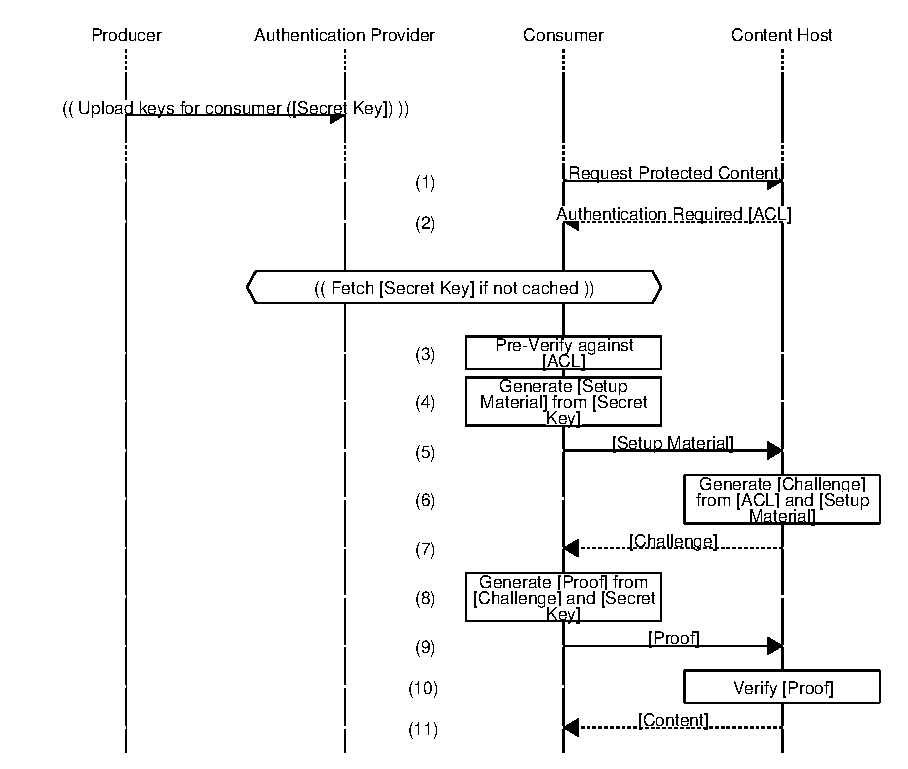
\includegraphics{auth.eps}
    \label{fig:auth}
    \caption{Authentication Protocol}
\end{figure}

Before running this protocol but after receiving the ACL, the consumer learns
the identity of the producer (listed in the ACL) and how many groups they are in
grant them access to the resource (this is simply an artifact of the crypto) but
not which ones. At this point, the content host learns nothing.

After running this protocol, the content host learns precisely that the consumer
has chosen to authenticate against an ACL.

\subsection{The Content Host's Perspective}

The previous section gives a top-down overview of the authentication protocol
but doesn't make it clear what the content host actually does. To keep it
simple, DRACL only exports two easy-to-understand functions to the content host:
\verb=is_acl= and \verb=authenticate=.

\verb=is_acl= simply verifies that an ACL is well formed. The content host
should use this function to verify that ACLs uploaded by producers are valid
(simply to avoid storing invalid ACLs).

\verb=check_access= takes an ACL and a response from the consumer and spits out
either \verb=GRANT=, \verb=DENY=, or \verb=CONTINUE(reply)= with a reply to be
sent to the consumer for further processing.

\subsection{The Consumer's Perspective}
\label{sec:consumer_perspective}

When attempting to access a protected piece of content, the browser first asks
the consumer if they want to prove that they have access and allows the consumer
to remember this decision (for the specific content host, for the specific
producer on this content host etc...). Additionally, if the consumer has never
seen the AP listed in the ACL before, the browser asks the consumer if it trusts
the AP. We do all this to prevent malicious parties from learning the consumer's
identity (see \cref{sec:doxing_consumers}). To make this less of a pain, we
expect browsers to ship with lists of trusted and untrusted APs and we tell the
consumer if the ACL has been signed by a producer they know (i.e., they have
previously shared/access content to/from them).

Finally, if the consumer's browser fails to generate the \verb=[Proof]=, it
warns the user. We do this to discourage content hosts from fingerprinting
consumers (see \cref{sec:fingerprinting}).

\section{Key Distribution}

In DRACL, consumers use secret keys (ACL Keys) given to them by producers when
authenticating to content hosts. This means they need some way of getting these
ACL Keys.

After choosing what groups each consumer should be in, the producer generates
one ACL Key for each consumer encoding the groups to which the consumer belongs
therein. The producer then encrypts the ACL Public Key with the consumer's
identity key, signs it with its own identity key, and uploads the encrypted ACL
Private Key, the associated ACL Public key, and the consumer's identity key to
the AP.

To download the ACL Key, the consumer asks the producer's AP for either all ACL
keys belonging to them (the consumer) or a subset thereof. When making this
request, the consumer proves that their identity key hasn't been revoked using
the identity system. Note, as the consumer identifies themself to the AP, the
browser should ask the consumer if they trust the AP.

\section{Account Compromise Recovery}
\label{sec:revoke}

DRACL supports account compromise recovery. When recovering a compromised
account, a user is able to restore the security of their account in case their
keys have been compromised. However, we don't currently support restoring
publisher privacy after a compromise as this would necessarily require updating
all old ACLs (see \cref{par:restore-privacy} for details). There are two parts
to account compromise recovery:

\begin{compactenum}
\item Account lockout.
\item Account restoration.
\end{compactenum}

In this section, we assume that the underlying identity system has a way of
marking identity keys as invalid/revoked. For example, the identity system could
attach a short-lived certificate to every identity key.

To support account lockout, (1) all ACL keys issued by DRACL expire rapidly (on
the order of hours) and (2) both the producer \emph{and} the producer's AP must
work together to make the ACL keys. This means that a compromise of either the
producer or the AP doesn't compromise the entire system.

To prevent an attacker with a compromised but revoked producer identity key and
from accessing that producer's content, we include a short-lived certificate
signed by the producer's AP in the ``setup material'' of the authentication
protocol (distributed along with the ACL Keys). If a producer notifies their AP
that their keys have been compromised, the AP will stop producing this
certificate effectively locking out all access to the producer's content.

To prevent an attacker with a compromised but revoked consumer identity key from
accessing content from other producers, we use a two-key system when
authenticating against ACLs. Basically, every ACL Key is actually two keys: one
issued by the producer that never expires and one issued by the producer's AP
that expires quickly. When the consumer goes to the producer's AP to ask for
their keys, they fetch both keys. When the consumer authenticates against an
ACL, they use both keys. This allows the producer's AP to revoke access to any
given consumer by simply not issuing its short-lived key. Importantly, the AP
can do so without help from the producer because the producer may be dead for
all we know.

To restore an account, we rely on the identity system. To support account
restoration, the underlying identity system must provide a mechanism for
securely transitioning from one (compromised) identity keypair to another.

However, after transitioning to a new key, users do not proactively replace old
ACLs as this would require additional work and implementation complexity for
content hosts. Instead, we continue to use the old ACLs as-is because our
system's security does not rely on any non-ephemeral secrets \emph{other} than
the identity key.

\chapter{Assessment}

Above all, we've designed DRACL to be implementable in practice, not only in
theory. Additionally, DRACL is privacy preserving, secure, and developer and
user friendly. Finally, as a decentralized system, DRACL promotes user-freedom.
This section evaluates how we stack up against our requirements for a ``good''
access control system for the web.

\section{Privacy Preserving}
\label{sec:privacy}

DRACL preserves the privacy of both producers and consumers. Preferably, DRACL
would reveal nothing other than whether or not some user should be able to
access some resource. Unfortunately, this goal is impossible to achieve given
our efficiency constraints. However DRACL provides reasonable privacy given our
performance constraints and some choices we've made when confronted with
unavoidable privacy/security trade-offs.

Perfect privacy is impossible given our performance constraints because not
doing something reveals that something hasn't happened. For example, because the
producer does not update ACLs after removing consumers from groups, a malicious
content host and consumer can collude to definitively learn that the consumer
has been removed from a group (because the ACL hasn't been updated so the group
structure must have been).

Below, we summarize what information DRACL reveals to the various parties involved:

\begin{description}
\item[Everyone] Every ACL includes the producer's public key so the content host
  and anyone attempting to access a resource learns something about the identity
  of the producer (see \cref{sec:producer_public} for why). This doesn't mean
  they learn the ``real'' identity of the producer but they do learn an
  identity. Additionally, anyone can learn whether or not a producer has put
  them in at least one group.
\item[Content Host] Content hosts know the content (which could be an encrypted
  blob) and learn whether or not a given (anonymous) consumer chooses to prove
  that they have access to piece of content.
\item[Consumers] Consumers learn whether or not they can access any resource at
  any point in time. However, they do not learn \emph{why} they have access.
  That is, they do not learn what groups they are in or what groups grant them
  access to any given resource. See section \cref{sec:resonable_privacy} for
  some caveats and exceptions (specifically, they learn how many groups grant
  them access).
\item[Authentication Providers] authentication providers learn their users'
  social networks but can't act on behalf of their users or access their
  content.
\item[Producer] An honest but curious producer cannot learn if and when specific
  friends access their content. Given sufficient collusion and effort, producers
  can learn something about who accesses what when but this is unlikely to be an
  issue in practice. See section the on consumer privacy
  (\cref{sec:consumer_privacy}) for details.
\end{description}

The following sections detail what privacy guarantees we provide and what
information we leak.

\subsection{Producer Privacy}
\label{sec:producer_privacy}

In general, DRACL provably reveals (almost, read on) nothing about the producers
social network to any third party other than the producer's AP (see
\cref{chap:crypto} for details).

\subsubsection{Reasonable Privacy}
\label{sec:resonable_privacy}

We have three privacy leaks that aren't entirely a result of some performance or
privacy trade-off.

First, consumers can learn how many of the groups they are in allow them to
access a resource. That is, given the set of groups a consumer is in,
$\mathbb{U}$, and the set of groups that can access a resource, $\mathbb{R}$,
the consumer can learn the size of the intersection, $|\mathbb{U} \cap
\mathbb{R}|$. This is simply an artifact of the cryptographic protocol we are
using for authentication. We believe we can fix this by using stronger (more
expensive) cryptographic primitives but haven't bothered exploring this avenue
because they're too inefficient. Furthermore we believe this should be fixable
without sacrificing performance but leave it to future work.

Second, anyone can learn whether or not an ACL has changed since the last time
they accessed a piece of content. In theory, one could randomize challenges so
that they look fresh every time. However this is likely more trouble than it is
worth as, for security reasons, we have content hosts present a signed copy of
the ACL along with challenges. Unfortunately, this does allow users to prove
that they have been added to or removed from some (but not which) group with
certainty by learning that they have gained/lost access to content without the
ACL changing. However, regardless of what we do, consumers can learn this with
high probability, but not with certainty, by simply assuming that gaining or
loosing access to a set of content is more likely to be the result of being
added or removed from a group than the result of each of those ACLs having been
changed in a short period of time.

Third, consumers can determine a lower bound on when an ACL may have been crated
because we record the ``time'' --- technically a monotonic counter, not the
actual time --- the producer last removed a consumer from a group before creating
an ACL in the ACL itself. This allows us to guarantee that all content published
\emph{after} a consumer is removed from a group is never accessible to that
consumer.

\subsubsection{The Producer Is Public}
\label{sec:producer_public}

In DRACL, the producer's public key is publicly visible in the ACL itself. This
may not be the producer's real identity, but it still identifies them. We had
four options:

\begin{compactenum}
\item List the producer (what DRACL does).
\item Allow ``friends'' to learn the identity of the producer. By ``friends'' we
  mean authorized consumers of \emph{some} content controlled by the producer.
\item Reveal the producer to the content host only.
\item Don't reveal the producer at all.
\end{compactenum}

It is provably impossible to implement option 4 without sacrificing
performance. Basically, because we don't update ACLs whenever a group definition
changes some party must use some producer-specific information at some point in
the authentication protocol. Because the AP can't participate directly in every
access check, this party must be either the content host or the consumer. We've
included a complete proof in \cref{proof:public-producer-4}

Implementing option 3 would either violate our security guarantees and open
content hosts up to denial of service attacks or force the producer to contact
every affected content host when their social network changes. As shown above,
either the content host or the consumer needs to learn the producer-specific
information. To prevent the consumer from learning the identity of the producer,
we'd either have to have the content host fetch this information from the
producer or have the producer send this information to the content host. The
first option violates our rule that the content host must never make network
requests on behalf of DRACL\@. As a matter of fact, this would be the worst case
scenario: the content host would be making a network request to a server
specified by a client (the producer) on behalf of a client (the consumer). On
the other hand, having the producer send the producer-specific information to
each content host ahead-of-time (whenever their social network changes) would
complicate the content hosts (they would have to listen for updates from an
external service) and force the producers to contact every content host they
have ever used whenever they change the members of one of their groups.

If we were to implement option 2, DRACL would either lose unidirectional
friendships or scale horribly at the tail. Basically, consumers could remember a
small list of producers with which they are actually friends. For each producer,
they could store a producer-specific secret that allows them to recognize an ACL
as having been authored by this producer. However, that would make it harder to
make new friends. In DRACL as designed, if a producer knows about a consumer,
they can grant that consumer access to content. If consumers had to pick a short
list of ``friends'' that could grant them access to content, we'd lose this
property.

On the other hand, consumers could keep track of every producer who has ever
shared a piece of content with them. Unfortunately, this would require them to
possibly keep track of many producers and require an infrastructure for
notifying consumers when a producer has shared some content with them.
Additionally, for popular users, this list could grow very large. Worse, the
size of this list scales based on actions taken by \emph{other} producers, not
the consumer in question. Finally, to actually authenticate against an ACL,
consumers would have to linearly search through the set of producer-specific
secrets to find the producer that authored the ACL\@. We sketch a proof for this
statement (making a reasonable assumption that we don't bother proving) in
\cref{proof:public-producer-2}.

In short, we make the producer public because it allows us to achieve better
usability and performance.

\subsubsection{The AP Learns The Social Network}
\label{sec:ap_learns_network}

In DRACL, APs learn the social networks of their producers. Specifically,
for any given producer, they learn which consumers that producer has put in at
least one group. However, they do not learn the group assignments.

This is a consequence of how we allow APs to revoke a consumer's access to a
producer's content without involving that producer. Basically, the AP needs to
be able to verify that the consumer's key has not been revoked when the consumer
fetches their keys; this identifies the consumer to the AP. Furthermore,
remember that the AP issues its own keys to consumers on behalf of its
producers. It needs to know for which producer it's issuing these keys so it can
properly sign them. This means that AP knows for and to whom it's issuing the
keys so it knows that the producer has put that consumer in a group.

One solution would be to have the producer's AP send consumers' keys to some
trusted broker (i.e., something like an AP but for consumers) and allow the
broker to know who the consumers are but not the producer's AP. This way, one
party (the broker) knows the consumer but not the producer, and the other party
(the AP) knows the producer but not the consumer. Unfortunately, this would
require a lot of up-front work and network traffic, even if the consumer never
views content published by some producer. By a lot, we mean that every time an
ACL key expires (on the order of hours) the producer's AP would have to send out
a ~30KiB key per consumer/producer relationship. Individually, this isn't much
data. However, assuming there are two equally popular APs, ACL keys expire twice
per day, and all producers have shared with 300 consumers on average over the
course of their existence, each AP would have to send 4MiB per producer to the
other AP twice a day. That's not that much data for active producers/consumers
but these data would have to be sent for inactive producers/consumers as well,
twice a day. On the scale of Facebook, that's 8PiB (that's \emph{Petabytes}) per
day.

However, this could be solved without adding a new party with some fancy crypto
and an anonymizing network. Basically (massive simplification), the producer
would get the AP to sign some keys where the consumer has been cryptographically
hidden (blinded) but the producer is visible (to the AP). Then, the producer
would unhide the part mentioning the consumer and hide the part mentioning the
producer and re-upload the altered key to the AP over an anonymous connection.
The consumer could now safely authenticate when downloading the keys because
they wouldn't be tied to the producer in any way (that part has been
cryptographically blinded). The consumer would then have to unhide the part that
mentions the producer to be able to successfully authenticate to content hosts.

Unfortunately, even the simplified this scheme above is complicated. It would
require a some fancy crypto (something like a partially blind partially
homomorphic signature algorithm), would require multiple rounds of communication
between the producer and their AP (some of them over anonymizing networks), and
would still be vulnerable to timing correlation attacks. By timing correlation
attack, we mean that, given that producer $A$ uploaded a key for signing at time
$T$ and an anonymous producer uploaded a key for consumer $B$ at time
$T+\epsilon$, $A$ is probably a friend of $B$.

Basically, a perfect system to hide the producer's social networks from APs but
such a system would be significantly more complicated.

\subsubsection{Recovery From Compromise}

If the producer's keys are compromised, their entire social network is leaked.
There's obviously nothing we can do about this. This is similar to a Facebook
account being hacked.

However, a problem specific to DRACL is that, after a producer's account has
been locked down from a security perspective, an attacker can still learn which
groups are members of (old) ACLs. This is an artifact of the fact that we do not
go back and replace old ACLs on account compromise. If the producer feels so
inclined, they could manually go back to every content host and replace their
old ACLs but we're not going to bake that feature into DRACL. Basically, we feel
that, at this point, the chicken has flown the coop so to speak.

\subsection{Consumer Privacy}
\label{sec:consumer_privacy}

DRACL allows consumers to anonymously access content. Specifically, DRACL
attempts to prevent content hosts and untrusted third parties from tracking
consumer behavior and browsing habits. However, there are ways in which
malicious parties can try to use DRACL to identify and/or track consumers in
some cases. Below we first discuss passive attacks that can let a content host
learn something about the identity of a consumer and then finish with an active
attack and some mitigations.

\subsubsection{Fingerprinting}
\label{sec:fingerprinting}

One problem with any access control scheme is that the content host can
fingerprint consumers based on what they can and cannot access. The consumer
could make every access request look like it's coming from a new client but this
is infeasible in practice. Instead DRACL allows the user to decide if and when
to authenticate and warns users (loudly) when authentication fails. This way,
consumers control what information they give to content hosts and content hosts
can only confirm answers they already suspect. While there are other ways for
content hosts to identify users (i.e., they could be logged in) DRACL should not
leak this information.

\subsubsection{Timing and Caching}
\label{sec:timing}

For increased performance and reliability, consumers cache keys retrieved from
producers. Unfortunately, caching tends to leak timing information. In our
case, we were worried that a curious content host could learn whether or not a
consumer ``knew'' a producer even if the consumer chose not to authenticate
based on whether or not the consumer had already cached the producer's key.

To mitigate this this, consumers pre-verify (\cref{sec:authentication}) if they
will be able to access a piece of content. If this pre-verification fails, they
never even initiate the authentication protocol. This means that the content
host can only possibly learn timing information if the user has access to the
content in question and has chosen to access it. However, in this case, the
producer already learns that the consumer ``knows'' the producer.

\subsubsection{Side Channels}

Content hosts will likely learn about the consumer's browser, IP address, etc.
This is beyond the scope of DRACL system and users that require true anonymity
should use the Tor Browser\cite{tor} or Tails\cite{tails}.

\subsubsection{Directly De-anonymizing Consumers}
\label{sec:doxing_consumers}

Unfortunately, consumers who habitually click ``yes'' for everything can be
trivially de-anonymized by a malicious content host. Here we discuss this
problem and our mitigations.

When fetching their keys from an AP, consumers must identify themselves to
properly handle consumer key revocation (see \cref{sec:revoke}). Unfortunately,
this means that an attacker (not necessarily a friend of the consumer!) can post
a resource to a content host along with an ACL that lists a unique AP domain
controlled by the attacker. If a consumer chooses to access this content,
they'll identify themselves (using the identity system) to this snoopy AP.
Because the domain is unique to the resource, the attacker learns that a
specific consumer has accessed a specific resource. This is obviously very bad.

To mitigate this, consumers only talks to trusted APs (see
\cref{sec:consumer_perspective}). Furthermore, because ACLs are signed by
producers, consumers can choose simply not authenticate against ACLs signed by
producers they don't recognize or trust. While a malicious producer could
deanonymize a user by tricking them into into using a malicious AP, we hope that
consumers in DRACL will have a better taste in friends.

There are a few alternatives:

\begin{enumerate}
\item Don't have the consumer identify to the producer's AP. Unfortunately, this
  means that the producer's AP can't verify that the consumer's key hasn't been
  revoked. We could provide an option for a consumer to claim: ``I know what I'm
  doing, I'll never lose control of my key.'' However, such ``expert only''
  options can be dangerous in practice so we would have to consider this very
  option carefully before adding it.
\item Push keys to the consumer's AP and have the consumer fetch them from
  there. This approach has already been discussed and refuted in section
  \cref{sec:ap_learns_network}.
\item Have consumers keep track of ``active'' friends and fetch ACL keys from
  them preemptively. This approach has already been discussed and refuted in
  section \cref{sec:producer_public}.
\end{enumerate}

So, malicious APs are a problem and consumers should avoid authenticating ACLs
from untrustworthy sources. At the end of the day, this is similar to not
logging into shady websites with something like Facebook Connect.


\section{User Friendly}
\label{sec:user_friendly}

We have designed DRACL (at the system level) to be user friendly and
unobtrusive. We meet our goals but there's still room for improvement.

\subsection{What We Got Right}

DRACL significantly reduces the cognitive burden on users and allows them to be
social on the web without performing tedious repetitive tasks.

Users only have to remember one set of credentials (their DRACL credentials).
DRACL can even be used to sign in to other systems by treating accounts as
resources. This, incidentally, also allows multiple people to share a single
``account'' without sharing passwords. We could probably go on-and-on about how
useful this is --- shared credentials are a big problem in the corporate world
--- but that's beyond the scope of this document.

Users can take their their social network with them from content host to content
host without giving up privacy.

Day to day, DRACL should be unobtrusive and integrate well with content hosts.
DRACL is designed to be implemented in the browser itself and to integrate
deeply with the browser. Unlike systems like OpenID, Facebook Connect, and
Google Sign-In, it won't have to open up a ``sign-in'' tab whenever the user
wants to authenticate, it can simply display a dialog box. Furthermore, on
content hosts a consumers uses regularly, when accessing content from producers
that the consumer ``knows'', the browser doesn't even have to ask the user to
authenticate. It can just silently authenticate on their behalf and display the
content (if instructed to do so by the consumer).

These last two issues have been cited~\cite{persona-fail} by Mozilla as reasons
reasons their authentication system, Persona, failed.

\subsection{Where We Could Improve}
\label{sec:usability_improve}

However, DRACL has some significant usability drawbacks: it's slow, revocation
isn't instantaneous, and the maximum number of consumers to which a producer can
grant access to content is limited (as it is on Facebook).

The client-side DRACL operations are \emph{very slow}. They take about 1-2
seconds on my 6 year old laptop so they should take at most a second on a recent
laptop. Worse, if a consumer has not accessed a piece of content from a producer
recently, they have to make a second round trip to that producer's AP to fetch
their keys. However, when compared to the time and effort it takes a user to
sign in to a website, this is actually quite cheep.

Revocation isn't instantaneous. This was discussed from a security standpoint in
section \cref{sec:secure} but it's really more of a usability problem. The UI
will have to make this clear to producers and warn them to manually re-create
ACLs for any content that they need to lock-down immediately. While unfortunate
from a usability standpoint, this problem is unavoidable given our requirements;
instantaneous revocation would require the AP to participate directly in the
authentication protocol.

Due to the crypto primitive we use, we have to limit the maximum number of
groups a producer can make. Unfortunately, our unit of access control is a
group; to share with an individual, you have to put them into an personal user
group. This means that the limit is effectively $g = |\mathit{groups}| +
|\mathit{consumers}|$. Currently, we've set this limit to 1000. We could
increase this limit but DRACL's keys, ACLs, and authentication protocol all
scale linearly with this constant. I get the following numbers on my laptop:

\vspace{2em}

\begin{tabular}{ >{\bfseries}r | >{$}r<{$} @{\quad$\approx$~} >{$}l<{$}}
  \hline
  Consumer Authentication Time & \unit[(.0015g + \epsilon)]{s} & \unit[1.5\pm .5]{s} \\
  Acl Size & \unit[(128g + \epsilon)]{B} & \unit[128]{KiB} \\
  \hline
  \multicolumn{2}{c}{} & \text{where } g=1000 \\
\end{tabular}

We believe these numbers can be improved simply by improving the underlying
cryptographic protocol. However, we leave that for future work.

Also, we don't currently provide a way to delete existing groups. However,
implementing this would be a straightforward improvement so we leave it to
future work. Basically, as ``dead'' groups accumulate, one would occasionally
transition to a new ACL Key (without the dead groups) and use the new key for
new content. This does mean that consumers would need every ACL Key ever created
by a consumer but, in practice, there shouldn't be that many. This is basically
a simple mark-compact garbage collection mechanism.

Overall, DRACL provides a large usability benefit over existing systems but our
security and performance requirements do impose a significant usability cost.

\section{User Freedom}

DRACL promotes user freedom through being decentralized, by allowing consumers to
freely move between content hosts, and by enabling developers to easily create
new services.

Simply by being decentralized, DRACL promotes user freedom by allowing producers
to choose their authentication provider.

By allowing producers to manage their social network through a single
authentication provider, DRACL allows users to carry their social network with
them from content host to content host. This reduces the barrier to moving
between content hosts and therefore promotes user freedom.

Finally, by allowing producers to share content with consumers on any content
host even if the consumer doesn't have an account at that content host, we've
reduced the difficulty of bootstrapping a new content host. This should make it
significantly easier for companies to break into the social network market which
should increase the number of social networks users can choose from.

One key missing component from our current design is the ability to move between
authentication providers. That is, we provide no simple way to migrate off one
AP to another. Adding this to DRACL should be relatively straightforward but it
would complicate an already complicated system.

Overall, DRACL promotes user freedom as much as possible while still remaining
practical.

\section{Secure}
\label{sec:secure}

DRACL is secure in practice. Being secure in some perfect world where all
software is perfect and bug free isn't practical. To this end, DRACL doesn't
allow unauthorized access to content (no exceptions), supports recovery from
account compromise, supports efficient revocation, and avoids being a vector for
denial of service attacks. DRACL's security is rooted in a standard CA system so
all \emph{security} compromises are recoverable as long as the CA system works.
This obviously isn't perfect because the CA system is deeply flawed but this can
always be replaced if and when a better alternative becomes available.

Only authorized users, the producer, and the content host are able to access
resources protected by DRACL\@. Specifically, DRACL doesn't allow the AP to
impersonate its users and access their content.

However, a malicious AP can time travel. That is, a malicious AP can revert any
consumer's view of any producer's social network to any previously valid state.
They can do this because the producer's ACL keys never expire (so that the
producer doesn't have to keep coming back online to re-sign them). In practice,
this means that a malicious AP can prevent a consumer from accessing content
they should be able to access and allow a consumer to access content that would
have been accessible to them in a previous incarnation of the producer's social
network in the content's current form (the AP can time-travel the social network,
not content). A security conscious producer can put an expiration date on
the ACL keys they issue to limit the effectiveness of such an attack but this
would force them to re-issue their ACL Keys before they expire to avoid locking
out access to \emph{all} their content.

Producers can efficiently revoke access to content. To facilitate this, DRACL
allows users to be removed from groups without updating every ACL mentioning the
now modified group. Much of the complexity of DRACL stems from this requirement.
Unfortunately, in order to do this efficiently, we sacrificed some security.
Specifically, content published by a producer before they remove a consumer from
a group will remain accessible to that consumer until their producer-specific
certificate expires. This is a more limited form of time-travel. We mitigate
this by making producer-specific certificates short-lived --- they expire on the
order of hours.

However, there is an important limitation on time travel in DRACL: consumers
with a time-traveled view of the social network --- either due to a malicious AP
or recently revoked access --- cannot access content published in later
incarnations of the social network. This is due to an epoch counter we include
in every ACL and every ACL Key. Basically, an ACL Key's epoch must be greater
than the ACL's epoch. A lower epoch indicates that the key is from an old view
of the social network and the content host will deny access.

Both consumers and producers are able recover and secure compromised accounts.
We achieve this by having APs act as semi-trusted third parties that certify
their user's keys with short-term certificates. Once an AP learns that one of
its users has been compromised, it stops signing their keys. The AP then works
with the user to transition the user to a new set of keys (authenticating the
user's identity out-of-band). For a quick overview of this protocol, see section
\cref{sec:authentication}.

\phantomsection
\label{par:restore-privacy}
Unfortunately, DRACL does not support restoring a producer's privacy after an
account compromise. That is, after an attacker obtains a set of ``producer
secrets'', they can determine what groups can access any given resource and, if
a consumer colludes with them, what groups that consumer is in.

DRACL stores \emph{no} sensitive information on the content host. This means
that, if a content host is compromised, they can simply restore from backup,
update their software, and continue on as if nothing happened --- as far as
DRACL is concerned at least.

The long-term security of DRACL rests entirely on the identity keys and the CA
system. To fully --- time travel doesn't count --- break the security of DRACL,
an attacker would have to obtain both the producer's identity key and a
certificate for AP's domain. The ``producer secrets'' are actually only secret
because they describe the producer's social network, not because they must
remain secret for security reasons.

Finally, DRACL cannot interfere with the operation of content hosts. To achieve
this, we guarantee that all DRACL operations performed by the content host will
complete in constant time. As a direct consequence of this, contents host never
initiate network requests on behalf of DRACL\@.

\section{Developer Friendly}

To be developer friendly, DRACL wraps all content-host logic in a simple
(interface wise), environment-agnostic library that should be easy to integrate
into existing content hosts. As noted in the system overview, we export three
functions: \verb=is_acl=, \verb=make_challenge=, and \verb=validate_response=.

First, these functions are dead simple. We expose no functionality beyond simple
access control checks. While more a complex interface may provide slightly better
efficiency through, e.g., caching, this would make it easier to misuse these
functions.

In addition to being simple, these functions perform \emph{no} network requests
and run in constant time (as noted in the security~\cref{sec:secure} section
above). This significantly reduces content host implementation complexity
because it means that these functions can be called synchronously.

Finally, access control checks never lead to database writes. This is important
for high-performance applications where reads are often performed out of
read-only caches.

However, DRACL isn't perfect from a developer's perspective. ACLs themselves are
approximately 128KiB, mostly due to our expensive crypto. This means that
developers will have to store a 128KiB binary blob somewhere. Furthermore,
verifying that a consumer has access to a piece of content requires that the
content host perform some reasonably expensive crypto. This crypto takes at most
a few milliseconds on modern hardware but that's still significantly more
expensive than, e.g., accessing an in-memory database.

\section{Scalable}

DRACL scales to the entire web. To achieve scalability, we put as little load on
the AP as possible.

APs aren't required to have perfect uptime. That is, in a steady state,
consumers can continue to access content and producers can continue to publish
content without having to contact the AP for every operation.

APs have storage and computation loads proportional to the number of
consumer-producer relationships, not proportional to the amount of content
published by a producer. Therefore, the cost of running a DRACL AP should scale
approximately proportionally to the number of users of the service. This means
that, a steady state, the cost of running an AP should actually decrease over
time as storage, bandwidth, and CPU power become cheaper.

DRACL is decentralized. This give instant scalability as the number of APs can
scale with demand.

However, it is unfortunate that APs need to do some crypto in real time when
consumers fetch their ACL keys. Currently, APs need to do some crypto when
handing out ACL Keys to consumers in order to verify that the consumer identity
key hasn't been revoked. However, we could do all the crypto offline
ahead-of-time using some fancier crypto schemes. Unfortunately, this gets a bit
complicated and may not be worth doing in practice. Regardless, this is worth
exploring as it would allow the AP to choose when and where to perform
moderately expensive computations which could significantly reduce the cost of
running an AP when compared to performing these computations on-demand.

\section{Future Work}

Throughout this chapter, we've identified future work that could improve DRACL.
Here, we list them off for easy picking.

\begin{itemize}
\item Don't leak the number of groups that grant a user access to a resource.
\item Look into allowing APs to perform all crypto off-line instead of
  on-demand.
\item Provide a way to garbage collect empty groups. To do this, producer would
  literally just transition to a new set of Producer Secrets (see
  \cref{sec:keys}) without defining the dead groups in the new secrets. However,
  there are some nuances that don't make this entirely trivial.
\item Cut out a round trip between the content host and the consumer. Currently,
  the consumer needs to send the content host some information before the
  content host can generate a challenge. This is actually only necessary for
  consumer anonymity, not security or producer privacy (see the anonymity
  proof). However it really should be possible to do this without the extra
  round; it's just non-obvious.
\item Increase the 1000 consumer/group limit and/or reduce our size/time complexity (\cref{sec:usability_improve}).
  \begin{itemize} 
  \item We believe that we could double this limit simply by improving the proof
    of the underlying crypto --- it doubles the size of the keys to make the
    proof go through but this may not be necessary.
  \item We have explored the possibility of making it possible to share with
    some number of groups and some (small) number of consumers directly. This
    way, we wouldn't have include the number of consumers in the 1000 group
    limit. However, this would require modifying the underlying cryptographic
    protocol and is non-trivial. By non-trivial, we mean that we don't know
    exactly how to do it but believe it to be possible. We could, with relative
    ease, allow granting access to some number of groups or (exclusive) an
    single consumer (identified by a unique ID) but this provides dubious
    benefit and complicates the underlying crypto (and may introduce some
    privacy issues, we haven't fully explored this option).
  \item We could provide some sort of hybrid scheme where producers have
    multiple sets of groups --- let's call them classes --- each with a 1000
    group limit. Consumers would be able to learn which classes they are a
    member of (e.g., ``MIT Student'', ``Class of 2014'', ``US Citizen'') but
    nothing about the actual group structure within the classes.
  \end{itemize}
\end{itemize}

\chapter{Authentication Protocol}

This chapter covers the authentication protocol itself assuming a few
cryptographic primitives which we describe in \cref{chap:crypto}.

\section{Primitives}

Before we can cover the authentication protocol, we need to know what tools we
can use.

\subsection{Standard Tools}

In the authentication protocol, we use standard tools like HMAC, hashing,
symmetric encryption, and asymmetric encryption. When we say encryption, we mean
authenticated encryption.

\subsection{Rerandomizable Signature Protocol}

TODO: Explain what this is.

\subsection{Encrypted Inner-Product Proof}

TODO: Explain this primitive.

\section{Setup}

TODO: use the primitives above here to make this clearer.

The ACL includes an encrypted bit-vector ($C$) that describes the groups
that should be granted access to the content and the consumer's ACL Private Key
($K$) includes another encrypted a bit-vector that encodes the groups in which
the consumer is a member. The consumer also has an ACL Public Key ($P$) along
with a certificate signed by the producer indicating the time period for which
$P$ is valid.

\section{Protocol}

TODO: use the primitives above here to make this clearer.

\begin{enumerate}
  \item The content host sends the ACL to the consumer along with a signature on
    the ACL signed by the producer.
  \item The consumer first verifies the signature on the ACL and decides whether
    or not to even attempt to authenticate against the ACL.
  \item They then pre-verify that they should be able to authenticate against
    the ACL by running the authentication protocol locally (pretending to be the
    content host).
  \item If they choose to continue, they then re-randomize their ACL Public Key
    (call it $P^r$) and sends it to the content host. This re-randomization
    ensures that the ACL Public Key does not uniquely identify the consumer.
    Note: We use a special signature scheme that allows the consumer to
    re-randomize their ACL public key while preserving the producer's signature
    on it.
  \item The content host verifies the signature on $P^r$ and verifies that it is
    currently valid (the key hasn't expired).
  \item The content host then ``mixes'' some secret $s$ into $C$ (we'll call
    this $C^s$), and uses the consumer's (randomized) ACL Public Key ($P^r$) and
    the ACL to compute some secret $Q^{rs} = f(C, s, P^r)$. $Q^{rs}$ has the
    crucial property that only someone who knows $P^r$ and either $s$ and $C$ or
    $C^s$ and a $K$ that (1) corresponds to $P^r$ and (2) intersects with $C$
    could determine.
  \item The content host computes $T = \hash(Q^{rs})$, and symmetrically
    encrypts $s$ using $T$ as the secret key to produce $E$.
  \item The content host then sends $E$ to the consumer along with $C^s$.
  \item The consumer computes $Q^{rs}$ from $C^s$, $P^r$, and $K$. They then
    hash it to recover $T$, and then decrypt $E$ to recover $s$.
  \item Now, the consumer re-creates $C^s$ from $C$ to verify that the content
    host followed the protocol correctly. This ensures that the content host
    can't fish for additional information by giving the consumer a malformed
    challenge (or one that doesn't correspond to the ACL presented in step 1).
  \item Finally, the consumer sends $\hmac(s, \text{``proof of membership for
      \texttt{domain\_of\_content\_host}''})$ back to the content host (where
    $\hmac$ is a keyed-hash message authentication code.
  \item The content host verifies the HMAC, verifies that the consumer knows
    what content host they are talking to to prevent man in the middle attacks,
    and finally grants them access to the content.
\end{enumerate}


\chapter{Crypto}
\label{chap:crypto}

\textit{A huge thanks to Prof. Vinod Vaikuntanathan (CSAIL, MIT) for extensive
  help (and hand-holding) while developing the crypto for DRACL.}

In DRACL, we needed a way for consumers to prove that the set of groups in which
they are a member intersects the set of groups that listed in an ACL. There are
three requirements that make this difficult:

\begin{enumerate}
\item These sets must remain secret from both parties. That is, we allow neither
  consumers nor content hosts to learn what groups the consumer is in nor what
  groups have access to any given resource.
\item The consumer needs to actually be able to prove to the content host that
  the vectors intersect \emph{without} identifying themself to the content host
  and/or granting the content host the ability to impersonate the consumer.
\item Consumers must lose the ability to prove membership after a period of
  time. That is, ACL Keys must expire.
\end{enumerate}

\section{Reduction To Math}
\label{sec:reduce-to-math}

To solve any problem with crypto, it must first be reduced to concrete math
(unless you have a ready-made crypto primitive that solves your problem for you
but we don't have that). In DRACL, every ACL includes a specially encrypted bit
vector of groups $\vec{a}$ that can access the content and every consumer is
given an encrypted bit vector of groups $\vec{b}$ in which they are a member
(the ACL Key). When authenticating, the consumer takes the inner product of
these two encrypted vectors, and, if the inner product is non-zero, the content
host grants them access. The tricky part is encrypting these vectors such that
the consumer can prove to the content host that the vectors have a non-zero
inner product without revealing anything more than that and that $\vec{b}$ has
not expired.

To hide the vectors, DRACL uses a function-hiding inner product encryption
scheme described by Bishop, Jain and Kowalczyk \cite{inner-product} along with
the privacy improvement described by Lin (in chapter 4)
\cite{inner-product-ext}.This allows us to compute an inner product of two
secret vectors without ever revealing anything about the vectors other than the
inner product.

\note{In this thesis, we ignore the privacy improvement
  (\cite{inner-product-ext}) because it's a black-box modification to the
  underlying protocol, doesn't actually affect any of our proofs, and adds
  unnecessary complication and noise. The extension is literally just: double
  the length of the encrypted vector and fill the extra space with zeros. An
  implementation will have to use this but it doesn't affect any of the proofs
  or explanations.}

\newcommand{\Ap}{\vec{\alpha}}
\newcommand{\Bp}{\vec{\beta}}
\newcommand{\ABp}{\iprod{\Ap}{\Bp}}

The details of this inner product encryption scheme are a bit messy so we're
going to abstract them away by defining a few functions. We define the functions
\allowbreak$\ein_1$, $\ein_2$, $\eins_1$, $\eins_2$, and $\eouts$. $\ein_i$
takes a length-two vector of cryptographic parameters and a vector to be
encrypted. $\eins_i$ just takes the cryptographic parameter vector without the
vector to be encrypted. $\eouts$ takes a scalar.

The inner product encryption scheme can (using a function $\pair$) combine
\allowbreak$\ein_1(\Ap, \vec{a})$ and \allowbreak$\ein_2(\Bp, \vec{b})$ to
produce $\eouts(\ABp\cdot\iprod{\vec{a}}{\vec{b}})$ where $\Ap$ and $\Bp$ are
the length-two parameter vectors and $\vec{a}$ and $\vec{b}$ are the vectors two
be encrypted. Additionally, one can combine (again, using $\pair$)
$\eins_1(\Ap)$ and $\eins_2(\Bp)$ to produce $\eouts(\ABp)$.

$\eins$, $\ein$, and $\eouts$ all have the following properties: 
\begin{enumerate}
\item The first argument is homomorphic over linear combinations. That is, there
  is a function $\combine$ that can produce $f(x\cdot \Ap + y\cdot Bp, \ldots) =
  \combine(x, y, f(\Ap, \ldots), f(\Bp, \ldots))$ assuming the remaining
  arguments are identical (where $f$ is one of the above functions).
\item The vectors passed into $\ein$ are ``hidden''. That is, given
  $\ein_1(\ldots, \vec{a})$ and $\ein_2(\ldots, \vec{b})$, it's possible to
  learn the inner product of these two vectors but nothing more. This was proven
  in \cite{inner-product} and \cite{inner-product-ext}.
\item Given $\ein_1(s \cdot \Ap, \vec{a})$, $\ein_2(\Bp, \vec{b})$,
  $\eins_1(\Ap)$, and $\eins_2(\Bp)$, it's hard to compute $\eouts(s\cdot\ABp)$
  unless $\iprod{\vec{a}}{\vec{b}}$ is non-zero. We prove this in
  \cref{sec:crypto-sec}.
\end{enumerate}

Now that we've abstracted away some of the underlying crypto, we can talk about
our actual authentication protocol.

\section{Authentication Protocol}

In this section, we discuss how we use the cryptographic tools introduced above
to build our authentication protocol.

\subsection{Basic Authentication Protocol}

Abstractly, the protocol is simple: the content host chooses a secret scalar
$s$, gives the consumer some encrypted form of $s$, and then gets back some form
of $s$ that the consumer wouldn't have been able to compute if
$\iprod{\vec{a}}{\vec{b}}$ were zero.

Below, we give a first attempt at the protocol and then fix some problems with
it in the following sections.

\subsubsection{Setup}

The producer includes $C_1 = \ein_1(\Ap, \vec{a})$ --- an encryption of
$\vec{a}$ --- and $C_2 = \eins_1(\Ap)$ in every ACL. In the consumer's ACL Key,
the producer includes $K_1 = \ein_2(\Bp, \vec{b})$ --- an encryption of
$\vec{b}$ --- as the ACL Private Key and $K_2 = \eins_2(\Bp)$ and a certificate
on $K_2$ --- certifying it as a valid ACL Public Key for some period of time --- as
the ACL Public Key.

\subsubsection{Protocol}

The content host sends the consumer the ACL ($C_1$, $C_2$). They (the consumer)
then computes:

\begin{align*}
  \eouts(\ABp)          &= \pair(\eins_1(\Ap), \eins_2(\Bp)) \tag{1} \\
                        &= \pair(C_2, K_2) \\
  \eouts(c \cdot \ABp)  &= \eouts(\ABp \cdot \iprod{\vec{a}}{\vec{b}}) \tag{2} \\
                        &= \pair(\ein_1(\Ap, \vec{a}), \ein_2(\Bp, \vec{b})) \\
                        &= \pair(C_1, K_1) \\
\end{align*}

If $\eouts(c \cdot \ABp)$ is $1$, authentication has failed and the consumer
aborts (this is the pre-verification step). Otherwise, they can brute-force $c$
because it must be small (it's the size of the intersection) by repeatedly using
$\combine$ on $\eouts(\ABp)$ ($\combine(\stackrel{\text{\tiny ?}}{c}, 0, \eouts(\ABp),
\eouts(\ABp))$).

Next, the consumer sends their ACL Public Key to the content host ($K_2$ and the
certificate on $K_2$) to the content host. The content host verifies the
certificate and verifies that $K_2$ is currently valid.

The content host then computes $C^s = \ein_1(s\cdot\Ap, \vec{a})$ and $R =
\pair(\eins(s\cdot \Ap),\,\eins_2(\Bp)) = \eouts(s\cdot \ABp)$. They send $C^s$
to the consumer and record $R$. The consumer then computes:

\begin{align*}
  \eouts(sc \cdot \ABp) &= \eouts(s \cdot \ABp \cdot \iprod{\vec{a}}{\vec{b}}) \tag{3} \\
                        &= \pair(\ein_1(s \cdot \Ap, \vec{a}), \ein_2(\Bp, \vec{b})) \\
                        &= \pair(\ein_1(s \cdot \Ap, \vec{a}), K_2) \\
\end{align*}

They then use $c$ and (3) to compute $\eouts(s\cdot\ABp)$ and prove to the
content host that they know this value (e.g., send it to them). Given propriety
3 from \cref{sec:reduce-to-math}, this would have been hard if the two vectors
had a non-zero inner product.

Unfortunately, $\Bp$ and, in-turn, $K_2$ uniquely identify the consumer which
violates our anonymity requirement.

\subsection{Anonymity}

To hide the consumer's identity, we randomize the consumer's ACL Public Key in
such a way that still allows the consumer to take the inner product between
$\vec{a}$ and $\vec{b}$. To do so, we give the consumer two keys that encode the
same vector but have different $\Bp$'s and allow them to take linear
combinations. Linear combinations randomize $\Bp$ and hide the user's identity.
That is, given:
\begin{align*}
  K_1 &= \ein_2(\Bp, \vec{b}) & K_2 &= \eins_2(\Bp) \\
  K^\prime_1 &= \ein_2(\Bp^\prime, \vec{b}) & K^\prime_2 &= \eins_2(\Bp^\prime)
\end{align*}
Compute (for some random $x$ and $y$):
\begin{align*}
  K^r_1 &= \ein_2(\iprod{x\Bp}{y\Bp^\prime}, \vec{b}) &= \combine(x, y, K_1, K_1^\prime) \\
  K^r_2 &= \ein_2(\iprod{x\Bp}{y\Bp^\prime}) &= \combine(x, y, K_2, K_2^\prime) \\
\end{align*}
And use $K_1^r$ and $K_2^r$ instead of $K_1$ and $K_2$.

\subsection{Expiration/Authenticity}

Unfortunately, now that we're allowing the user to take linear combinations of
their keys, we can't just sign $K_2$ (because the consumer never gives $K_2$ to
the content host). Instead we need a homomorphic signature scheme that allows
consumers to take linear combinations of (the parameters of) $K_2$ while
preserving the signature.

Luckily, Signatures For Network Coding\cite{signature} proposes a scheme that
almost gives us what we want. The specific scheme proposed assumes that the
vectors will be in the clear, not encrypted like in our scheme. However, some
modifications make this scheme work with DRACL. We don't discuss them here
because the details rely on the specific definitions of the abstract functions
we've been using.

% Luckily, we were able to modify an existing homomorphic signature scheme created
% for something called network coding (described in \cite{signature}) to fit our
% needs. You can read \cref{sec:homo-sig} if you want to know how this signature
% scheme works.

TODO: LINK TO SECTION

\subsection{Two Factors}

Another problem with this scheme is that we want to allow the consumer to
authenticate with two keys: one signed by the AP and the other signed by the
producer (refer to \cref{sec:revoke}).

Recall that we're storing all these keys on the producer's AP and the consumer
is fetching them as needed. The ACL Private Key is encrypted so the AP can't
mess with it however, we don't need to encrypt the ACL Public Key.

So, we can have the AP take two linear combinations of $K_2$ and $K_2^\prime$
($K^{(AP)}_2$ and $K^{(AP)\prime}_2$), sign them, and then give them to the
consumer along with a description of the linear combination the AP took.

After the consumer downloads their keys, they can can take the same linear
combinations of their $K_1$ and $K_1^\prime$ to get $K^{(AP)}_1$ and $K^{(AP)\prime}_1$.

Now, the consumer can authenticate twice: once with each of these keys.

\subsection{Less Crypto}

At this point, we have everything we need. However, we can cut the (really
expensive) crypto done by the client by a third. Recall, the client currently
takes the inner product of the encrypted vectors 3 times: once for
pre-verification, twice for authentication (once for each key). However, given
that these vectors are actually just linear combinations of each other and we're
allowed to take linear combinations, we can combine the AP's and producer's keys
into a single key and authenticate with it in one go.

Basically, we make the following changes.

\begin{enumerate}
\item Content host: Instead of using $K_2^r$ and $K^{(AP)~r}_2$
  separately, the content host adds them together to produce a single
  $K_2^{(combined)} = \combine(1, 1, K_2^r, K^{(AP)~r}_2)$ (after verifying the certificates, of course).
\item Consumer: The consumer adds together both ACL Private Keys ($K_1^r$ and
  $K^{(AP)~r}_1$) and then uses them as a single $K_1^{(combined)} = \combine(1,
  1, K_1^r, K^{(AP)~r}_1)$.
\end{enumerate}

\subsection{Tearing Down The Abstraction}

Finally, we can tear down our abstraction. Luckily, it maps directly to the
underlying function-hiding inner product encryption crypto.

First, whenever we have vectors in exponents of groups, we mean a vector of
groups to the elements of the vector. That is, $g_i^{\vec{v}} = (g_i^{v_1},
g_i^{v_2}, \ldots, g_i^{v_n})$.

Then, given the vectors $\vec{d}$, $\vec{d^\star}$, $\vec{b}$, and $\vec{b^*}$
as described in \cite{signature} and a bilinear pairing function $\e$, the
functions we've been using map to the underlying crypto protocol as described in
\cref{fig:abstraction}.

\begin{figure}[H]
\label{fig:abstraction}
\begin{align*}
  \eins_1(\Ap) &= g_1^{\alpha_1\vec{d^*}_1 + \alpha_2\vec{d^*}_2} && \text{; In \cite{signature}, $\alpha_1 = \alpha$ and $\alpha_2 = \tilde{\alpha}$.} \\
  \eins_2(\Bp) &= g_2^{\beta_1\vec{d}_1 + \beta_2\vec{d}_2} && \text{; In \cite{signature}, $\beta_1 = \beta$ and $\beta_2 = \tilde{\beta}$.} \\
  \ein_1(\Ap, \vec{x}) &= g_1^{\alpha_1\left(\sum_{x_i \in \vec{x}}{_i\vec{b^*}_i} + \vec{b^*}_{2n+1}\right) + \alpha_2\left(\sum_{x_i \in \vec{x}}{x_i\vec{b^*}_i} + \vec{b^*}_{2n+3}\right)} \\
  \ein_2(\Bp, \vec{x}) &= g_2^{\beta_1\left(\sum_{x_i \in \vec{x}}{_i\vec{b}_i} + \vec{b}_{2n+1}\right) + \beta_2\left(\sum_{x_i \in \vec{x}}{x_i\vec{b}_i} + \vec{b}_{2n+3}\right)} \\
  \pair(a, b) &= \e(a, b) \\
  \eouts(a) &= \e(g_1, g_2)^a \\
  \combine(x, y, g_i^{\vec{u}}, g_i^{\vec{v}}) &= \left(g_i^{\vec{u}}\right)^x \cdot \left(g_i^{\vec{v}}\right)^y = g_i^{x\vec{u} + y\vec{v}}
\end{align*}
\caption{Cryptographic Abstraction}
\end{figure}


%\section{Homomorphic Signature Scheme}
%\label{sec:homo-sig}
%
%We use a variant of~\cite{signature} to allow consumers to re-randomize their API
%public key while still preserving security.
%
%Given a set of sets of vectors encoded in the exponents of a group in a bilinear
%map, our scheme allows an administrator to sign each set of vectors such that a
%user that knows one or more sets of these vectors can take a single set of
%vectors and produce a signed linear combination of this set of vectors. However,
%
%\begin{enumerate}
%\item It is computationally infeasible to produce valid signatures on linear
%  combinations of vectors belonging to different sets.
%\item Anyone who knows the source set for a combined vector can determine the
%  linear combinations of vectors that produced this combined vector.
%\item Given a set of vectors known to have the same source set and a test
%  vector, it is computationally infeasible to determine if the test vector
%  belongs to the source (without knowing the source).
%\end{enumerate}
%
%Essentially, this is an unlikable signature scheme with a trap door.
%
%\subsection{Construction}
%
%Given a vector size of $n$, the set of vectors and signatures are constructed as
%follows:
%
%First, pick some secret $t$ and add $T = \e(P_{n+1}, Q)^t$ to the public key.
%
%Then for the $i^{\mathit{th}}$ vector $\vec{v}$ in the set of vectors to sign,
%pick a random number from the group $a_i$ and compute:
%
%\begin{align*}
%  \vec{u} &= \left(P_{1}^q, \underbrace{P_{j+1}^{v_j},\dots}_{ 1 \le j \le n}, \middle| \underbrace{0\ldots, 0,}_{i-1 \text{ zeros}} a_i, \underbrace{0\dots, 0,}_{n-i \text{ zeros}}\right) \\
%  o &= Q^{\frac{1}{q}} \\
%  \sigma &= \underbrace{\prod_{i=1}^{n+1}{u_i^{s_i}}}_{\text{already in the exponents}} \prod_{i=n+2}^{2n+1}{P_i^{s_i u_i}} \\
%\end{align*}
%
%Unlike the original scheme, we store some of the components (those before the
%bar) in the exponents instead of in the clear. This means that they don't need
%to be put into the exponent when verifying the signature.
%
%To verify the signature, follow the original scheme (subject to the modification
%above) and then check that $e(u_1, Q) == T$. This ensures that linear
%combinations can only be taken within a single set of vectors.
%
%To take a linear combination within a set of vectors ($u^\prime$), take a linear
%combination of the entries before the bar in the exponent and the same linear
%combination of the entries after the vertical bar normally. Then, take the
%linear combination of the signatures as one would do in \cite{signature}.
%
%Finally, compute the new $o^\prime = o^{\frac{1}{\sum_{i}{c_i}}}$ where each
%$c_i$ is a coefficient used in the linear combination produced in the previous
%step. This way, $e(u_1, o)$ still equals $T$.

\begin{appendices}

\chapter{API}
\label{chap:api}

This chapter covers how to use DRACL as a content-host developer.

\section{Server Side API}

We expose two functions as a part of the server-side API.

\begin{compactitem}[$\lambda$]
\item \verb=is_acl(acl) -> bool= \\
  Validates that the ACL is well-formed. The content host should call this
  method before storing an ACL to catch errors up-front.
\item \verb=check_access(server_secret, origin, acl, response) -> Challenge= \\
  Runs a round in the authentication protocol.

  The parameters are:

  \begin{description}[labelindent=2em,leftmargin=4em]
  \item[\texttt{server\_secret}] \hfill \\
    A server-specific symmetric secret key. This needs to stay the same for the
    course of the authentication protocol (multiple rounds of communication)
    however, it can be re-used everywhere. Your web framework likely already
    \emph{has} a global server secret. Just use that one.
  \item[\texttt{origin}] \hfill \\
    The content host's origin. This allows the content host to verify that the
    no-one is performing a man-in-the-middle attack on the consumer.
  \item[\texttt{acl}] \hfill \\
    The ACL.
  \item[\texttt{response}] \hfill \\
    An opaque \texttt{response} from the consumer
  \end{description}

  It returns one of:

 \begin{description}[labelindent=2em,leftmargin=4em]
 \item[\texttt{Grant(until)}] \hfill \\
   Grant the consumer access until \texttt{until}. The \texttt{until} field
   dictates until when the content host should grant access. This allows content
   hosts to to record, in a cookie for example, how long the user should be
   granted access to the resource without having to re-authenticate.
 \item[\texttt{Continue(challenge)}] \hfill \\
   Return \texttt{challenge} to the consumer.
 \item[\texttt{Deny}] \hfill \\
   Deny access.
 \end{description}
\end{compactitem}

\subsection{Client Side API}

The client-side API uses JavaScript. We'd liked to have supported a variant that
uses HTTP-Auth headers but, unfortunately, the challenge object used in DRACL is
large ($\approx\unit[128]{KiB}$) and simply wouldn't fit in an HTTP header.
Fortunately, the response object is tiny (end-users tend to have little upstream
bandwidth).

The client exposes several functions:

\begin{compactitem}[$\lambda$]
\item \verb=authenticate(challenge, callback: function(response))= \\
  This function takes an opaque challenge blob (or the ACL if this is the first
  round of authentication). It calls callback if the consumer decides to
  proceed.

  \note{\texttt{callback} will never be called if the user chooses to not
    authenticate. See section \cref{sec:timing}.}

  The \texttt{response} argument to \texttt{callback} should be sent back to the
  server and run through the server-side \texttt{check\_access} function.
\item \verb=create_acl(description, callback: function(acl))= \\
  Ask the browser to create an ACL. The \texttt{description} parameter is a human
  readable description of the purpose of this ACL.
\item \verb=edit_acl(acl, callback: function(acl))=
  Asks the browser to modify an ACL. This is how a producer edits who can access
  a piece of content.
\end{compactitem}

\subsection{Authentication Protocol}

From the developer's perspective, the protocol works as follows:

\newcommand{\server}{\underline{\texttt{server}}}
\newcommand{\client}{\underline{\texttt{client}}}

\begin{compactenum}
\item The consumer attempts to access a piece of content protected by an ACL.
\item \server{} The content host returns the ACL to the consumer's browser as
  \texttt{challenge}
\item \client{} The content host calls \texttt{authenticate} in the
  consumer's browser:
  \begin{verbatim}
authenticate(challenge, function(response) {
  /* ... */
});
\end{verbatim}
\item \client{} When and if the callback executes, it should return
  \texttt{response} to the content host.
\item \server{} On the content host, call \verb=check_access(secret, origin, acl, resp)=.
\item \server{} If the result is \texttt{Deny}, abort.
\item \server{} If the result is \texttt{Continue(challenge)}, send \texttt{challenge}
  back to the consumer's browser and go back to step 3.
\item \server{} If the result is \texttt{Grant(until)}, grant access until the
  time specified by \texttt{until}.
\end{compactenum}

Importantly, the server maintains no mutable state.

\chapter{Proofs}

\emph{Gandalf: Fly, you fools!}

\section{Consumer Anonymity}

In this section, we prove our anonymity requirement. Specifically, we prove that
the content learns nothing more than whether or not the consumer has access to a
piece of content. We assume that neither the producer nor the AP collude with
the content host. Otherwise, this would be theoretically unprovable for any
access control system as the producer could create an ACL that grants access to
precisely one consumer.

First, the consumer re-randomizes their ACL Public Key before authenticating so
the content host cannot identify the consumer though this public key. As a
matter of fact, the re-randomization mechanism we use information theoretically
hides the consumer's identity. The consumer re-randomizes their ACL Public Key
by taking linear combinations of two length-two linearly independent vectors. As
these vectors are linearly independent, they form a basis and a random linear
combination of any two of these vectors is truly random.

Second, it's impossible for the content host to learn anything other than
whether or not the given consumer is listed in the ACL because they can't cheat
in the authentication protocol. Basically, they can ask a single question (``are
you (the consumer) a member of this ACL?'') signed by the producer and learns
the hash of the secret that was used to generate the challenge. Proof: recall
that after successfully generating a challenge-response, the consumer learns the
secret that the content host used when generating the challenge. Also recall
that the consumer learns the ACL (signed by the producer). This means that the
consumer can re-create the challenge and verify that it was created correctly
(well, that it could have been created correctly).

This tells the content host precisely that the consumer was able to extract the
secret from the challenge (the bit that indicates that the user should be
granted access) and nothing more (they already must have known the secret to
produce the challenge).

Therefore, at the end of the authentication protocol, the content host learns
only that the consumer is a member of the ACL.

{\hfill $\square$}

\section{Producer Privacy}

In this section, we prove privacy. That is, we prove that DRACL hides the
structure of its producers' social networks from third parties. Specifically, we
prove that no party can directly learn which groups are listed in any given ACL or
which groups a consumer is a member of (although consumers can learn the size of
the intersection between their groups and those listed in an ACL).

Proof: This follows directly from the guarantee given by the underlying
function-hiding inner product encryption scheme \cite{inner-product}: the
function-hiding inner product encryption scheme reveals nothing about the
``functions'' (vectors) except their inner products (the size of the
intersection).

{\hfill $\square$}

\section{Security}
\label{sec:crypto-sec}

In this section, we prove that DRACL is secure. That is, no party can convince a
content host that they are listed in an ACL unless they have an ACL Private Key
whose group set intersects with the ACL's group set and an associated ACL Public
key with a valid certificate.

\subsection{Assumption}

To prove security, we assume that computing $\e(g_1, g_2)^{abc}$ is hard given:

\begin{flalign*}
g_1, g_1^a, g_1^b, g_1^c, g_1^{c^{-1}} \\
g_2, g_2^a, g_2^b, g_2^c, g_2^{c^{-1}} \\
\end{flalign*}

This is a variant on the standard SXDH assumption.

\subsection{Theorem}

Given all information known by parties other than the content owner
\emph{except} the set of private keys whose group vectors intersect some set of
target ACLs chosen by the attacker, it is hard for an attacker to prove against
any of the target ACLs.

Specifically, the attacker can:

\begin{itemize}
  \item Pick which groups can access which resources ($\mathbf{X}$) and which
    users are in which groups ($\mathbf{Y}$), both described by binary vectors.
  \item Pick some set of target ACLs against which they intend to prove access.
  \item Know all ACLs.
  \item Know all user public keys and all public key generators for all epochs.
  \item Know all user secret keys for all epochs \emph{except} those valid in the current epoch.
  \item Know all user secret keys valid in current epoch \emph{except} those that grant access to the target ACL.
\end{itemize}

\subsubsection{Reduction}

Assume there exists a function $f$ that can take all of the information listed
above and return a proof of access against the target ACL.

There exists an efficient reduction from the security assumption to $f$:

First, let:

\begin{align*}
  g_2^t &= g_2^a & g_1^{sq} &= g_1^b \\
  g_2^{q^{-1}} &= g_2^c & g_1^{q} &= g_1^{c^{-1}}
\end{align*}

Then: \\

\begin{enumerate}
\item Pick $\mathbf{X} = \{\vec{x}_i\}$ (where each vector describes the groups
  that have access to a resource) and $\mathbf{Y} = \{\vec{y}_i\}$ (where each
  vector describes the groups in which a consumer is a member) 
  such that there exists some inner product $\iprod{\vec{y}_i}{\vec{x}_j} = 0$
  (some consumer does not have access to some resource).
\item Pick some non-empty set of vectors $\mathbf{X_\tau}$ of
  $\mathbf{X}$ to represent the ACLs of the target resource(s).
\item Let $\gamma$ be the set of groups the attacker is a member of in the
  current epoch. Choose a subset $\mathbf{Y_{\upsilon}}$ of the vectors in
  $\mathbf{Y}$ that have a zero inner products with the rows in
  $\mathbf{X_\tau}$. \emph{not} a member. $\gamma = \{ j ~ | ~ \exists~\vec{y}
  \in \mathbf{Y_\upsilon}.~\vec{y}_i[j] = 1 \}$ (i.e., the attacker is a member
  in the $j^{\mathit{th}}$ group in one of their ACL keys).
\item Pick $\mathbb{D}, \mathbb{D^*} \leftarrow
  \dual(\mathbb{Z}_p^2)$, and $\mathbb{B^\prime}, \mathbb{B^{\prime *}} \leftarrow
  \dual(\mathbb{Z}_p^{2n+4})$ as described in the paper. 
  $(\mathbb{B^\prime}, \mathbb{B^\prime *})$ are the same as $(\mathbb{B},
  \mathbb{B^\prime *})$ as described in the paper except that the vectors that
  match the groups that the attacker is not in are scaled by a factor of
  $q^{-1}$.
\item Generate all ACLs in the system: For each vector in $\mathbf{X}$,

  \begin{enumerate}
  \item Pick $\alpha$, $\tilde{\alpha}$ as described in the paper.
  \item Let \begin{flalign*}
      C_2 &= g_1^{\alpha\vec{d_1^*} + \tilde{\alpha} \vec{d_2^*}} \\
      C_1 &= \left(g_1^q\right)^{\alpha\left(\sum_{\forall x_i \in \vec{x} | i \in \bar{\gamma}}{x_i\vec{b^*}_i}\right) + \tilde{\alpha}\left(\sum_{\forall x_i \in \vec{x} | i \in \bar{\gamma}}{x_i\vec{b^*}_i}\right)} \\
        &\times \left(g_1\right)^{\alpha\left(\sum_{\forall x_i \in \vec{x} | i \in \gamma}{x_i\vec{b^*}_i} + \vec{b^*}_{2n+1}\right) + \tilde{\alpha}\left(\sum_{\forall x_i \in \vec{x} | i \in \gamma}{x_i\vec{b^*}_{n+i}} + \vec{b^*}_{2n+3}\right)}
    \end{flalign*}
  \end{enumerate}
\item Generate the target challenges:
\item Let \begin{flalign*}
      C_{s} &= \left(g_1^{sq}\right)^{\alpha\left(\sum_{x_i \in \vec{x}}{x_i\vec{b^*}_i} + \vec{b^*}_{2n+1}\right) + \tilde{\alpha}\left(\sum_{x_i \in \vec{x}}{x_i\vec{b^*}_i} + \vec{b^*}_{2n+3}\right)}
  \end{flalign*}
\item Generate keys for all epochs other than the current one.
  \begin{flalign*}
    K_2 &= g_2^{\beta\vec{d_1} + \tilde{\beta}\vec{d_2}} \\
    K_1 &= \left(g_2^{-q}\right)^{\alpha\left(\sum_{\forall y_i \in \vec{y} | i \in \bar{\gamma}}{y_i\vec{b}_i}\right) + \tilde{\alpha}\left(\sum_{\forall y_i \in \vec{y} | i \in \bar{\gamma}}{y_i\vec{b}_i}\right)} \\
        & \times \left(g_2\right)^{\alpha\left(\sum_{\forall y_i \in \vec{y} | i \in \gamma}{y_i\vec{b}_i} + \vec{b}_{2n+1}\right) + \tilde{\alpha}\left(\sum_{\forall y_i \in \vec{y} | i \in \gamma}{y_i\vec{b^*}_{n+i}} + \vec{b}_{2n+3}\right)} \\
  \end{flalign*}


\item Generate keys for the current epoch for all consumers in
  $\mathbf{Y_{\upsilon}}$ where $\beta = t\cdot \beta^\dagger$ and $\tilde{\beta} =
  t\tilde{\beta^\dagger}$:
  \begin{flalign*}
    K_2 &= \left(g_2^t\right)^{\beta^\dagger\vec{d_1} + \tilde{\beta^\dagger}\vec{d_2}} \\
    K_1 &= \left(g_2^t\right)^{\beta^\dagger\left(\sum_{y_i \in \vec{y}}{y_i\vec{b}_i} + \vec{b}_{2n+1}\right) + \tilde{\beta^\dagger}\left(\sum_{y_i \in \vec{y}}{y_i\vec{b}_i} + \vec{b}_{2n+3}\right)} \\
    \\
    K_2^\prime &= \left(g_2^t\right)^{\beta^\dagger\vec{d_1} + \tilde{\beta^\dagger}\vec{d_2}} \\
    K_1^\prime &= \left(g_2^t\right)^{\beta^\dagger\left(\sum_{y_i \in \vec{y}}{y_i\vec{b}_i} + \vec{b}_{2n+1}\right) + \tilde{\beta^\dagger}\left(\sum_{y_i \in \vec{y}}{y_i\vec{b}_i} + \vec{b}_{2n+3}\right)} \\
  \end{flalign*}

\item First pick a random $o_1$ and $o_2$ as the homomorphic secret key for the
  current epoch and then generate the public key: $P = g_1^{(o_1,o_2)}$.

\item Pick a random $s_1$ and $s_2$ for the signature scheme and homomorphically
  sign the $K_2$'s for the current epoch:
  \begin{flalign*}
    \sigma(K_2) &= K_{2_1}^{o_1} \cdot K_{2_2}^{o_2} \\
    \sigma(K_2^\prime) &= {K^\prime_{2_1}}^{o_1} \cdot {K^\prime_{2_2}}^{o_2}
  \end{flalign*}
\end{enumerate}

We feed all $K_1$'s and $K_2$'s, all $C_1$'s and $C_2$'s, all challenges
($C_s$), the homomorphic public key ($P$), and the signatures on $K_1$'s from
the current epoch ($\sigma(K_1$).

To break our scheme, $f$ would have to produce $R = \e(g_1, g_2)^{s \cdot
  \iprod{(\alpha, \tilde{\alpha})}{\vec{z}}}$, and some $K^{(t)}_{2} =
(g_2)^{\vec{z}}$ where $\vec{z}$ is some length two vector. Additionally, it
would have to signature $\sigma_k = \sigma(K^{(t)}_2)$ such that $\e(K^{(t)}_2,
P) == \sigma_k$ (i.e., the signature verifies).

Recall that, given the homomorphic signature scheme we're using, it's
computationally infeasible to compute a signature on a vector though any means
other than taking linear combinations of existing vectors. Therefore, $f$ must
have produced $P$ (and the signature) by taking linear combinations of some set
of $K_2$'s from the current epoch (these are the $K_2$s signed by the current
key).

Therefore, if $f$ exists, there must exist some function $f^\prime$ that take
the same parameters as $f$, and, instead of yielding $\sigma_k$ and the
signature on it directly, yields the set of linear combinations that was used to
produce $\sigma_k$ and the signature.

So, instead of reducing to $f$, we reduce to $f^\prime$.

Also recall that all $K_2$'s from the current epoch have a $t$ in the exponent.
This means that $P = (g_2)^{\vec{z}} = (g_2^t)^{\vec{z^\prime}}$ for some
$\vec{z^\prime}$. This also means that $R = \e(g_1, g_2)^{s \cdot
  \iprod{(\alpha, \tilde{\alpha})}{\vec{z}}} = \e(g_1, g_2)^{st \cdot
  \iprod{(\alpha, \tilde{\alpha})}{\vec{z^\prime}}}$.

Given that we know the linear combination of $K_2$'s that went into $K^{(2)}_t$
and we chose all the components in the exponent of these $K_2$s \emph{except}
for $t$, we can trivially compute $\vec{z^\prime}$. Additionally, we also know
all the $\alpha$ and $\tilde{\alpha}$ parameters that went into this black box
so we can brute force $(\alpha, \tilde{\alpha})$ in polynomial time. Therefore,
we can compute $\iprod{(\alpha, \tilde{\alpha})}{\vec{z^\prime}}$ and remove it
from the exponent of $R$. This leaves us with $\e(g_1, g_2)^{st}$ which is the
same thing as $\e(g_1, g_2)^{st}$. However, this violates our original
assumption so the function $f^\prime$ cannot exist. This, in turn, means that
$f$ cannot exist.

{\hfill $\square$}

\section{The Producer Is Public Proofs}

This section is simply a set of expanded proofs for the claims we made in
\cref{sec:producer_public}.

\subsection{Option 4 Is Provably Impossible}
\label{proof:public-producer-4}

Here, we prove that option 4 from \cref{sec:producer_public} is impossible to
achieve in any protocol that meets DRACL's performance requirements. Forgetting
DRACL, assume there exists a system that meets the requirements of DRACL. This
system must avoid updating individual ACLs when the members of a group change
(requirement 1). This system must avoid contacting a third party such as the AP
while authenticating (requirement 2). To achieve the first requirement, the ACLs
must not fully specify who has access to what (there must be some indirection).
Therefore, there must be some additional information needed for authentication
that describes the current state of the producer's social network (i.e., what
consumers are in what groups). Additionally, this information must be specific
to the producer (it describes the producer's social network). To achieve the
second requirement, this additional information must be reusable between
authentication attempts against multiple ACLs because only the consumer and the
content host are allowed to participate in the authentication protocol.
Therefore, given an ACL known to have been authored by some producer and another
ACL authored by an unknown producer, either the consumer or the content host
(the only participating parties) must learn whether or not the second ACL was
authored by the same producer as the first simply because it will reuse the same
producer specific information.

{\hfill $\square$}

\subsection{Option 2 Requires A Linear Search}
\label{proof:public-producer-2}

We asserted that the producer would have to linearly search through a list of
producer-specific secrets to provide guarantee 2, here we give a proof sketch
(with an assumption) of why we believe this to be true. Basically, the ACL would
have to include some constant-sized tag that only an authorized consumer could
recognize. To be constant-sized, it can't describe the list of consumers that
should be able to recognize it (would require infinite compression). Therefore,
this information has to be distributed among the consumers (it has to exist
somewhere). Therefore, every consumer would have some tag-recognition key from
that corresponds to each producer known by that consumer (issued independently
because this is a decentralized system). Furthermore, each of these tags would
have to look random and unique to avoid identifying the producers to third
parties. Finally, we'd need some form of polynomial-time algorithm that can
convert a polynomial size list of such tag-recognition keys into a function
(e.g., something like a hash map) that maps tags to tag-recognition keys in time
sublinear in the number of tag-recognition keys. We assume that no such
algorithm can exist because it would have to exploit some pattern or structure
in these necessarily random tags.

{\hfill $\square$}

\chapter{Spec}

This section is simply an implementation recipe. You should \emph{only} read
this if you actually want to implement DRACL. If you just want to understand it,
read the System Overview (\cref{chap:system-overview}). If you just want to use
it on your content-host, go back to the API ( \cref{chap:api}).

\section{Keys}

First, we need to understand the different types of keys in this system:

\begin{description}
\item[Consumer/Producer Identity Key] The consumer and producer both have
  asymmetric identity key pairs. These are plain-old PGP keys that are used by
  the consumer, producer, and AP but \emph{not} the content host. If possible,
  these should be stored on a secure element.
\item[AP Key] Every AP has a standard SSL certificate issued by a trusted CA.
\item[ACL Key] This is a special asymmetric key (using our custom crypto) that
  consumer's use to access a producer's content. There are two parts: the ACL
  Public Key and the ACL Private Key. While producers issue individual ACL
  Private Keys to each of their friends, they issue a single ACL Public Key;
  otherwise, content hosts would be able to identify the consumer based on this
  public key. Again, as explained in the overview, there are actually two ACL
  Keys: one issued by the producer and one by the producer's AP
\item[Producer Secret] Every producer has a set of secrets used to generate ACLs
  and ACL Keys.
\end{description}

\section{Datastructures}

Here, we define the datastructures that DRACL uses. For convenience, we encode
all messages and datastructures in CBOR. A more efficient encoding (e.g.
Protocol Buffers) could be used at a future stage.

Note: All numbers encoded as \texttt{bytes} are encoded in network order.

\subsection{Common Data Structures}

Below, we define a few common data structures that we'll need throughout the
protocol.

First, we define a \texttt{type} field simply to make introspection easier.

\subsubsection{\texttt{SignedEnvelope}}

We define a \texttt{AuthenticatedEnvelope} type for encapsulating authenticated messages:

\begin{leftbar}
\begin{description}
\item[\texttt{type}] \verb="authenticated"=
\item[\texttt{data}] \texttt{bytes} \\
  The authenticated data.
\item[\texttt{auth}] \texttt{bytes} \\
  The signature/MAC.
\end{description}
\end{leftbar}

When we use \verb=authenticated(data)= in the following message definitions, we
mean that the data ``data'' is wrapped in a signed envelope with
signature/message authentication code ``auth''. Note: we don't specify the
specific key, method, or type because \emph{how} a message should be verified
depends on the internals.

\subsubsection{\texttt{EncryptedEnvelope}}

We define a \texttt{EncryptedEnvelope} type for encrypting messages:
\begin{leftbar}
\begin{description}
\item[\texttt{type}] \verb="public_key"=
\item[\texttt{encrypt\_type}] \verb="pgp"= \\
  The encryption format. Currently, only \verb="pgp"= is supported.
\item[\texttt{data}] \texttt{bytes} \\
  The encrypted data.
\end{description}
\end{leftbar}

When we use \verb=encrypted(enc_key, data)=, we mean that the data is first
wrapped in a signed envelope, then an encrypted envelope. The key that's needed
to decrypt \texttt{data} should be encoded in \texttt{data} (how this is done is
up to the underlying encryption system).

\subsubsection{\texttt{PublicKey}}

We define a \texttt{PublicKey} type for describing public keys:

\begin{leftbar}
\begin{description}
\item[\texttt{type}] \verb="public_key"=
\item[\texttt{key\_type}] \verb="PKCS12"= (DER encoded), \verb="RSA"= (DER
  encoded RSA key), or \verb="PGP"= (binary format) Opaque key data (in the case
  of PKCS12, this contains the entire certificate chain).
\item[\texttt{key}] \verb="key"= \\
  The actual key data.
\end{description}
\end{leftbar}

\subsubsection{\texttt{Name}}

Finally, we define a \texttt{Name} type for identifying public keys. These allow
indirection so that the actual underlying public key can change.

\begin{leftbar}
\begin{description}
  \item[\texttt{type}] \verb="name"=
  \item[\texttt{name\_type}] \verb="dns"=, \verb="pgp"=, or "rsa"
    \begin{compactdesc}
    \item[\texttt{dns}] A domain name. An associated public key would be the full
      certificate chain (X.509) signed by a trusted root CA.
    \item[\texttt{pgp}] A PGP key fingerprint. TODO: Subkeys, key transitions...
    \item[\texttt{rsa}] A DER encoded RSA public key.
    \end{compactdesc}
  \item[\texttt{name}] \texttt{bytes}
    The actual name.
\end{description}
\end{leftbar}

\subsection{\texttt{ACL}}

Below is the specification for the internal format of an \texttt{ACL}.

\begin{leftbar}
\begin{description}
\item[\texttt{type}] \verb|"acl"|
\item[\texttt{acl\_key\_authorities}] \verb=[Name]= \\
  A set of names that map to the keys that need to have signed the ACL keys used
  to authenticate against this resource. That is, a consumer will need a
  non-expired ACL Key signed by each of the parties listed below.
  
  In general, this will list the AP's domain and producer's RSA key (using the
  RSA format, not PGP).
  
  For technical reasons, these can't be PGP names. Basically, we don't want to
  require PGP on the hosts.

\item[\texttt{producer}] \texttt{Name} \\
  The producer's identity (using the identity system).
  
  This is used by the consumer to learn the identity of the producer. This is
  also the key used to sign the ACL.

\item[\texttt{producer\_ap}] \texttt{string} \\
  The producer's AP (where to find the necessary keys).

\item[\texttt{epoch}] \texttt{u64} \\
  An monotonically increasing integer used to prevent
  time travel. See the discussion for details.

\item[\texttt{acl\_v1}] \texttt{bytes} \\
  The current ACL format. Versioned in case we decide to change the underlying
  crypto. See the crypto section (\cref{chap:crypto}) for more.

\item[\texttt{user\_data}] \texttt{any} \\
  Small opaque user-data blob (should be symmetrically encrypted by the
  producer). This allows the producer to record information about the ACL in the
  ACL itself (e.g., a description of the groups/users listed in the ACL).
\end{description}
\end{leftbar}

\texttt{SignedACL} is defined to be an ACL wrapped in a signed envelope (signed
by the producer).

\subsection{ACL Keys}

\subsubsection{\texttt{ACLPrivateKey}}

\begin{leftbar}
\begin{description}
\item[\texttt{type}] \verb="acl_private_key"=
\item[\texttt{public\_key\_fingerprint}] \texttt{bytes} \\
  A SHA256 hash of the associated ACLPublicKey. Not necessary but can't hurt.

\item[\texttt{comment}] \texttt{string} \\
  A short comment written by the producer for the consumer. This is effectively a MOTD.
\item[\texttt{epoch}] \texttt{u64} \\
  This key is only valid for ACL's with epochs less than or equal to \texttt{epoch}.
\item[\texttt{secret\_v1}] \texttt{bytes} \\
  The actual secret key. See the crypto specification (\cref{sec:crypto-spec})
  for more.
\end{description}
\end{leftbar}

\subsubsection{\texttt{ACLPublicKey}}

\begin{leftbar}
\begin{description}[labelindent=2em,leftmargin=3em]
\item[\texttt{type}] \verb="acl_public_key"=
\item[\texttt{signing\_key}] \texttt{PublicKey} \\
  The public key that signed this ACL Key. Can either be an RSA key or a
  full PKCS12 key+certificate chain.

\item[\texttt{expires}] \texttt{u64} \\
  Unix timestamp when this key expires.

  In general, the producer's ACL Public Key will never expire (that's why we
  have an AP) but the AP's Public Key should expire on the order of a few
  hours.
  
  Zero means never.

\item[\texttt{public\_v1}] \texttt{bytes} \\
  The public part of the crypto protocol (see \cref{sec:crypto-spec}).
\end{description}
\end{leftbar}

\subsection{Authentication Protocol Data Structures}

\subsubsection{\texttt{Challenge}}

\begin{leftbar}
\begin{description}
\item[\texttt{type}] \verb="challenge"=
\item[\texttt{crypto\_challenge\_v1}] \texttt{bytes} \\
  The actual challenge as defined by the crypto protocol.
\item[\texttt{user\_data}] \texttt{any} \\
  Some extra data included by the content host. This will be returned along with
  the \texttt{ChallengeResponse} and is used to avoid having to keep state on
  the content host.
\end{description}
\end{leftbar}

\subsubsection{\texttt{ChallengeResponseBody}}
\label{struct:challenge_response_body}

\begin{leftbar}
\begin{description}
\item[\texttt{type}] \verb="challenge\_response\_body"=
\item[\texttt{origin}] \texttt{string} \\
  The server from which this request originated (authenticated by a secure
  channel such as TLS). This allows the server to detect MITM attacks.
\item[\texttt{crypto\_response\_v1}] \texttt{bytes} \\ 
  The actual challenge as defined by the crypto protocol.
\item[\texttt{user\_data}] \texttt{any} \\
  The extra data included in the challenge from this response was generated.
\end{description}
\end{leftbar}

\subsubsection{\texttt{ChallengeResponse}}
\label{struct:challenge_response}

TODO authenticated...

\begin{leftbar}
\begin{description}
\item[\texttt{type}] \verb="challenge\_response"=
\item[\texttt{}] \texttt{bytes} \\ 
  The actual challenge as defined by the crypto protocol.
\item[\texttt{user\_data}] \texttt{any} \\
  The extra data included in the challenge from this response was generated.
\end{description}
\end{leftbar}

\section{Crypto Internals}
\label{sec:crypto-spec}

TODO: Explain encoding for the ``crypto'' parts. We store them as raw bytes and
decode them manually for ultimate storage efficiency.

\end{appendices}

\bibliographystyle{acm}
\bibliography{thesis}

\end{document}
% vim: set foldmethod=marker: %
